% !TeX spellcheck = en_US
%\documentclass[preprint,authoryear]{elsarticle}
\documentclass[preprint]{elsarticle}
% sudo apt-get install -y texlive-publishers

\usepackage[left]{lineno}
\usepackage[latin1]{inputenc}
\usepackage[T1]{fontenc}
\usepackage{lmodern}
\usepackage{multirow}

\usepackage{lineno,hyperref}
\modulolinenumbers[5]

\usepackage[none]{hyphenat}

\usepackage{url}
\usepackage{booktabs}

\usepackage{tikz}
\usetikzlibrary{calc}
\usetikzlibrary{positioning}

\usepackage{mathtools}
\usepackage{amssymb}
\usepackage{amsthm}

\usepackage{caption}
\captionsetup{labelfont=bf}
\captionsetup{skip=0pt}

\usepackage{pgfplots}
\pgfplotsset{compat=newest}
\usepackage{algorithm}

\usepackage[noend]{algpseudocode}

\usepackage[margin=0.9in]{geometry}

\usepackage[normalem]{ulem}
%\usepackage{xcolor}

\newcommand{\Comentar}[1]{\State {\cmmt{#1}}}
\newcommand{\Break}{\State \textbf{break}}
\renewcommand{\Return}{\State \textbf{return}~}
\renewcommand{\algorithmicensure}{\textbf{Parameters:}}

\renewcommand\algorithmicthen{}
\renewcommand\algorithmicdo{}


\algblock{ForEach}{EndFor}
\algblock{ForDownTo}{EndFor}
\algblock{ForTo}{EndFor}

\newcommand{\Block}[1]{\State #1 \{}
\newcommand{\EndBlock}{\State \}}

\usepackage{scrextend}
\newcommand{\boldm}[1] {\mathversion{bold}#1\mathversion{normal}}
\newcommand{\round}[1]{\ensuremath{\lfloor#1\rceil}}
\usepackage{setspace}
\usepackage{array}
\usepackage{color, colortbl}
\definecolor{Gray}{gray}{0.9}
\hyphenation{cost-ef-fec-tive-ness}

\newcommand{\specialcell}[2][c]{%
	\begin{tabular}[#1]{@{}c@{}}#2\end{tabular}}


\journal{Computers \& Industrial Engineering}


\begin{document}


\begin{frontmatter}

\title{Air cargo load and route planning in pickup and delivery operations}

\author{A.C.P.~Mesquita}
\ead{celio@ita.br}

\author{C.A.A.~Sanches\corref{cor1}}
\ead{alonso@ita.br}
\cortext[cor1]{Corresponding author.}

\address {Instituto Tecnol\'{o}gico de Aeron\'{a}utica - DCTA/ITA/IEC\\
Pra\c{c}a Mal. Eduardo Gomes, 50\\
S\~{a}o Jos\'{e} dos Campos - SP - 12.228-900 - Brazil}


\begin{abstract}

In aerial pickup and delivery of goods in a distribution network, transport aviation faces risks of cargo unbalancing due to the urgency required for loading, for fast take-off, and mission accomplishment, especially in times of crisis, disaster relief missions, short deadlines for contracting customers, or any external pressure for immediate take-off. {\color{blue} In addition, there are no commercially available systems that can assist the load and trip planners with the pallet building and aircraft loading and balancing demands for transport at each hub.} This enables other risks, such as improper delivery, excessive fuel burn, and longer than necessary turn-around time. We defined and solved the problem of planning the loading and routing of an aircraft according to a utility score, weight and balance principles, and fuel consumption in a tour of simultaneous pickup and delivery at intermediate hubs. This NP-hard problem, named {\it Air Cargo Load Planning with Routing, Pickup, and Delivery Problem (ACLP+RPDP)}, is mathematically modeled using standardized pallets in fixed positions, obeying center of gravity constraints, delivering each item to its destination, and minimizing fuel consumption costs. We performed multiple experiments with a commercial solver and four well-known meta-heuristics on data based on the transport history of the {\it Brazilian Air Force}. We also designed a new heuristic that quickly finds good solutions for a wide range of problem sizes: an essential contribution, which solved all test scenarios within an acceptable operational run time.


\end{abstract}

\begin{keyword}
Load Planning \sep Air Palletization \sep Weight and Balance \sep Pickup and Delivery \sep Vehicle Routing
\end{keyword}

\end{frontmatter}

\label{sec1}
\section{Introduction}


Air cargo transport involves several sub-problems that are difficult to solve. Recently, Brandt and Nickel \cite[p. 401]{BrandtStefan2019} defined the {\it Air Cargo Load Planning Problem} (ACLPP) as four sub-problems: {\it Aircraft Configuration Problem} (ACP), {\it Build-up Scheduling Problem} (BSP), {\it Air Cargo Palletization Problem} (APP) and {\it Weight and Balance Problem} (WBP). Several aspects were considered in this modeling: characteristics of the items to be transported (dimensions, scores, dangerousness, etc.); types and quantities of {\it unit load devices} (ULDs), commonly called pallets; when these pallets are assembled; how items are allocated to pallets; in which positions these pallets are to be placed; how the total cargo weight is balanced; etc. They also presented a comprehensive bibliographic survey of solving methods that had been developed in different situations.

However, there are still other important challenges in air cargo transport that go beyond the definition of the ACLPP, especially with regard to the flight itinerary and the loading and unloading at each destination (or node) of this travel plan. In this context, at least two more important sub-problems can be considered: pickup and delivery operations at each node, called {\it Pickup and Delivery Problem} (PDP), and the search for the lowest cost route, which is the well-known {\it Traveling Salesman Problem} (TSP).

Considering air cargo transport, Table \ref{tab:sa} lists the main works in the literature and the corresponding sub-problems addressed. We also indicate whether the dimensions of the items were taken into account ({\bf 3D} or {\bf 2D}) and which solution method {\color{blue}was used: heuristic search methods ({\bf Heu}), integer programming ({\bf Int}), or linear programming ({\bf Lin}).}

\begin{table}[H]
	\centering
	\caption{Air cargo transport: literature, problems and features}  \label{tab:sa}
	\scriptsize
	\renewcommand{\arraystretch}{1.1} 
	\begin{tabular}{r|cccc|ccccc}
		\toprule
		 Work & {\bf APP}  & {\bf WBP}  &  {\bf PDP}   &{\bf TSP}   & {\bf 2D}  & {\bf 3D}  & {\bf Heu}  & {\bf Int}  & {\bf Lin} \\
		\midrule
		Larsen and Mikkelsen \cite{LarsenMikkelsen1979}  & $.$        & $\bigstar$ & $.$          & $.$        & $.$       & $.$       & $\bigstar$ & $.$        &  $.$ \\
		Brosh \cite{Brosh1981}  & $.$ & $\bigstar$  & $.$   & $.$ & $.$ & $.$   & $.$  & $.$  &  $\bigstar$ \\
		Ng \cite{Kevin1992}  & $.$ & $\bigstar$  & $.$ & $.$ & $.$ &$.$   & $.$  & $\bigstar$  &  $.$ \\
		Heidelberg {\it et al.} \cite{Heidelberg1998}  & $.$ & $\bigstar$  & $.$ & $.$ & $\bigstar$ &$.$   & $\bigstar$  & $.$  &  $.$ \\
		Mongeau and Bes \cite{MongeauBes2003}    & $\bigstar$ & $\bigstar$   & $.$ & $.$ & $.$ & $.$   & $.$  & $\bigstar$  &  $.$ \\
		Fok and Chun \cite{fok2004optimizing} & $.$ & $\bigstar$   & $.$ & $.$ & $.$ & $.$   & $.$  & $\bigstar$  &  $.$ \\	
		Chan {\it et al.} \cite{Chan2006}  & $\bigstar$ & $.$    & $.$ & $.$ & $.$ & $\bigstar$  & $\bigstar$  & $.$  &  $.$ \\
		Kaluzny and Shaw \cite{KaluznyBohdanL2009Oalb}  & $.$ & $\bigstar$  & $.$  & $.$ & $\bigstar$ &$.$  & $.$  & $\bigstar$  &  $.$ \\
		Verstichel {\it et al.} \cite{Verstichel2011}   & $.$ & $\bigstar$    & $.$ & $.$ & $.$ & $.$   & $.$  & $\bigstar$  &  $.$ \\
		Mesquita and Cunha \cite{MesquitaCunha2011}   & $.$ & $.$    & $\bigstar$ & $.$ & $.$ & $.$   & $\bigstar$  & $.$  &  $.$ \\		
		Limbourg {\it et al.} \cite{Limbourg2012} & $.$ & $\bigstar$  & $.$ & $.$ & $.$ & $.$   & $.$  & $\bigstar$  &  $.$ \\
		{\color{blue}Roesener and Hall} \cite{RoesenerHall2014}  & $\bigstar$ & $\bigstar$  & $.$  & $.$ & $.$ & $\bigstar$   & $.$  & $\bigstar$  &  $.$ \\
		Vancroonenburg {\it et al.} \cite{Vancroonenburg2014}  & $\bigstar$ & $\bigstar$   & $.$ & $.$ & $.$ & $.$   & $.$  & $\bigstar$  &  $.$ \\
		Lurkin and Schyns \cite{LurkinSchyns2015} & $.$ & $\bigstar$  & $\bigstar$ & $.$  & $.$ & $.$   & $.$  & $\bigstar$  &  $.$ \\
		Roesener and Barnes \cite{RoesenerBarnes2016}  & $.$ & $\bigstar$   & $.$ & $.$ & $.$ & $.$   & $\bigstar$  & $.$  &  $.$ \\
		Paquay {\it et al} \cite{PaquaySchynsLimbourg2016,PaquayLimbourgSchynsOliveira2018}  & $\bigstar$ & $\bigstar$ & $.$ & $.$ & $.$ & $\bigstar$ & $\bigstar$  & $\bigstar$ & $.$ \\
		Chenguang {\it el al.} \cite{YangLiuGao2018} & $.$ & $\bigstar$  & $.$  & $.$ & $\bigstar$  & $.$ & $\bigstar$ & $.$  & $.$ \\
		Wong and Ling \cite{wong2020} & $\bigstar$  & $\bigstar$  & $.$  & $.$   & $.$  & $.$ & $.$ & $\bigstar$  & $.$  \\
		Wong {\it et al.} \cite{eugene2021} & $\bigstar$ & $\bigstar$ & $.$  & $.$   & $.$ & $.$ & $.$ & $\bigstar$  & $.$  \\
		Zhao {\it et al.} \cite{zhao2021} & $.$ & $\bigstar$ & $.$  & $.$  & $.$ & $.$ & $.$  & $\bigstar$ &  $.$ \\
		{\bf This article}   & $\bigstar$ & $\bigstar$  & $\bigstar$& $\bigstar$ & $.$ & $.$ & $\bigstar$ & $\bigstar$   &  $.$  \\
		\bottomrule 
	\end{tabular}
	\normalsize 
\end{table}


As can be seen, so far Virginie Lurkin and Micha�l Schyns \cite{LurkinSchyns2015} is the only work that simultaneously addresses an air cargo (WBP) and a flight itinerary (PDP) sub-problem. Although it is innovative, strong simplifications were imposed by the authors: in relation to loading, APP was ignored; with regard to routing, it is assumed a pre-defined tour plan restricted to two legs. It is important to note that these authors consider an aircraft with two doors, and the minimization of loading and unloading costs at the intermediate node was modeled through a container sequencing problem. Referring directly to this work, Brandt and Nickel \cite[p. 409]{BrandtStefan2019} comment: {\it However, not even these sub-problems are acceptably solved for real-world problem sizes or the models omit some practically relevant constraints}. 

There are real situations that are much more complex. In this work, we consider a practical case in Brazil, which is the largest economy in Latin America. Due to its dimensions, this country has the largest air market on the continent with $2,499$\/ registered airports, of which $1,911$\/ are private and $588$\/ are public. Although it is an immense distribution network, airlift missions consider 3 to 5 nodes per tour plan. Throughout this work, we address routes with up to 7 nodes, as can be seen in Table \ref{tab:costs} and Figure \ref{fig:nodes}.

{\color{blue} 
	This 7-node limitation is more than enough for the case of the {\it Brazilian Air Force}. In case some extension is needed for this range, a more suitable TSP solution method may be adopted, as full enumeration may make it impractical for other clients' real-world scenarios.
}


\begin{table}[H]
	
	\begin{minipage}{0.05\linewidth}
		
	\end{minipage}\hfill 
	\begin{minipage}{0.45\linewidth}
		
		\caption{Brazilian airports distances ($km$)}  \label{tab:costs}
		\centering
		\footnotesize
		\newcolumntype{Y}{>{\centering\arraybackslash}p{0.09\textwidth}}
		\newcolumntype{X}{>{\centering}p{0.09\textwidth}}
		
		\begin{tabular}{X X X X X X X Y}
			\toprule
			Node & $l_0$ & $l_1$ & $l_2$ & $l_3$ & $l_4$ & $l_5$ & $l_6$ \\
			IATA*   & GRU   & GIG   & SSA   & CNF   & CWB   & BSB   & REC \\	
			\midrule	
			GRU     & 0	    &343	&1,439   &504    &358    &866    &2,114\\
			GIG	    & 343	&0	    &1,218   &371    &677    &935    &1,876\\
			SSA	    & 1,439	&1,218	&0	    &938    &1,788   &1,062   &676\\
			CNF	    & 504	&371	&938	&0	    &851    &606    &1,613\\
			CWB	    & 358	&677	&1,788	&851	&0	    &1,084   &2,462\\
			BSB	    & 866	&935	&1,062	&606	&1,084	&0	    &1,658\\
			REC	    & 2,114	&1,876	&676	&1,613	&2,462	&1,658	&0\\
			\bottomrule
			\multicolumn{8}{c}{*International Air Transport Association}\\
			\multicolumn{8}{c}{\small\textsuperscript{Source: www.airportdistancecalculator.com}}\\
		\end{tabular}
		\normalsize
		
	\end{minipage}\hfill 
	\begin{minipage}{0.50\linewidth}
		\centering
		\includegraphics[scale=0.25]{Images/nodes.png}
		\captionof{figure}{A route with some Brazilian airports}
		\label{fig:nodes}		
	\end{minipage}
\end{table}

{\color{blue} 
	
	Although there are many other airports in the Brazilian Air Force's interest, these seven were chosen due to their huge demands and short lead times for transportation, which are worthy of aerial transportation. The other airports may have a lower transportation demand, which is frequently less costly to address by cabotage, railways, or road transport�as well.
}

In the {\it Brazilian Air Force}\/ missions, hundreds of items can be carried at each node, where the objectives are to prioritize the transport of the most important items and minimize the cost of fuel along the route. As standardized pallets are used with predefined positions on the aircraft, it is possible to carry out loading and unloading at each node in around 30 minutes{\color{blue}, if the pallet's position and contents are already planned}.

{\color{blue}
As to the cargo item arrangement on the pallets as well as the route planning, which normally takes two hours, which is the same time reported by Kelly Fok and Andy Chun \cite{fok2004optimizing} "the container load planning is usually done in roughly 2 hours before departure, when all cargo details are in place.", it is essential to find a way to shorten this time to improve the efficiency of cargo transportation. However, there are no commercially available systems or software packages that can simultaneously solve these problems.
}


\begin{table}[H]
	
	\begin{minipage}{0.05\linewidth}
		
	\end{minipage}\hfill 
	\begin{minipage}{0.40\linewidth}
		
	{\color{blue}	
Cargo handling at modern airports usually involves powerful equipment like dollies, powered conveyors, elevating transfer vehicles, caster decking, scissor lifts, electrical controls, hydraulically adjustable heights, forklift trucks, and plenty of room in the airport cargo terminal.

\vspace{3mm}
These facilities can help with a complete pallet re-arrangement in the cargo bay, if necessary, in less than 30 minutes if the pallet position contents are already planned.
}
		
	\end{minipage}\hfill 
	\begin{minipage}{0.55\linewidth}
		\centering
		\includegraphics[scale=0.2]{Images/handling.png}
		\captionof{figure}{Cargo handling equipment}
		\label{fig:handling}
			
		\small\textsuperscript{Source: NARA \& DVIDS Public Domain Archive}	
	\end{minipage}
\end{table}



This work proposes a method that {\color{blue}addresses} these objectives: a pallet building and arrangement plan with a routing option that maximizes the benefit-cost ratio for the smooth execution of pickup and delivery transport missions.

We develop a heuristic that can be executed on a simple handheld computer (like a laptop or a tablet) and that provides a solution quickly enough to keep this cargo handling time {\color{blue}under 30 minutes.} This heuristic {\color{blue} solution certainly will} reduce the stress that transport planners are subjected to, because they have to deal with a lot of information in planning the aircraft route, assembling the pallets ({\color{blue}regarding their positions), and a pick up and delivery plan to each node.}

To the best of our knowledge, this is the first time that an air cargo transport problem that simultaneously involves APP, WBP, PDP and TSP has been addressed. This new problem is named {\it Air Cargo Load Planning with Routing, Pickup and Delivery Problem} (ACLP+RPDP).

This article is organized into six more sections. In Section \ref{sec2}, we give a brief review of the literature. In Section \ref{sec3}, we present the problem context and assumptions, and in Section \ref{sec4}, we describe the mathematical model and how we dealt with its issues. In Section \ref{sec5}, we describe the elaborate algorithms, whose results are presented in Section \ref{sec6}. Finally, our conclusions are in Section \ref{sec7}.



\section{Related literature}
\label{sec2}

In this section, we briefly describe the characteristics of the main works related to air cargo transport, following the chronological order of Table \ref{tab:sa}.

Ole Larsen and Gert Mikkelsen \cite{LarsenMikkelsen1979} developed an interactive procedure for loading 14 types of Boeing 747 into a two-leg transportation plan. Seven types of items were considered to be allocated in 17 to 42 positions. With non-linear programming and heuristics, they present a solution that minimizes positioning changes in the intermediate node, optimizing the load balancing in the aircraft.

Israel Brosh \cite{Brosh1981} addressed the problem of planning the allocation of cargo on an aircraft. Considering volume, weight and structural constraints, the author finds the optimal load layout through a fractional programming problem.

Kevin Ng \cite{Kevin1992} developed a multi-criteria optimization approach to load the {\it C-130} aircraft of the {\it Canadian Air Force}. Based on integer programming, this model provides timely planning and improves airlift support for combat operations, solving WBP with pallets in fixed positions, and considering 20 different items.

Heidelberg {\it et al.} \cite{Heidelberg1998} developed a heuristic for 2D packing in air loading, comparing it with methods for solving the {\it Bin Packing Problem}. These authors conclude that the classical algorithms are inadequate in this context, because they ignore the aircraft balancing constraints.

Marcel Mongeau and Christian Bes \cite{MongeauBes2003} presented a method based on linear integer programming to solve the problem of choosing and positioning containers in the {\it Airbus 340-300}. Safety and stability constraints were considered, with the objective of minimizing fuel consumption.

Kelly Fok and Andy Chun \cite{fok2004optimizing} developed a web-based application to make efficient use of space and load balancing for an air cargo company. Based on an analysis of historical data, an operational load planning with mathematical optimization is obtained. This container load planning is usually done in roughly 2 hours before departure, when all cargo details are in place.

Chan {\it et al.} \cite{Chan2006} carried out a case study with heterogeneous pallets. To minimize the total cost of shipping, they developed a 3D packing heuristic, with a loading plan for each pallet. Although the authors do not consider load balancing or positioning of pallets in the cargo hold, this method is relevant in commercial and industrial applications, where cargo items tend to be less dense.

Bohdan Kaluzny and David Shaw \cite{KaluznyBohdanL2009Oalb} developed a mixed integer linear programming model to arrange a set of items in a military context that optimizes the load balance. {\color{blue}The objective function can be chosen to minimize the deviation of the center of gravity from the target position or to maximize the function of the items loaded. This approach does not palletize items, which are arranged in the cargo bay by a 2D packing procedure.
}

Verstichel {\it et al.} \cite{Verstichel2011} solved WBP by selecting the most profitable subset of containers to be loaded into an aircraft by the use of mixed-integer programming. Experimental results on real-life data showed significant improvements compared to those obtained manually by an experienced planner.

Mesquita and Cunha \cite{MesquitaCunha2011} presented a heuristic for a real problem of the {\it Brazilian Air Force}, which consists of defining transport routes with simultaneous collection and delivery from a central distribution terminal.

Limbourg {\it et al.} \cite{Limbourg2012} developed a mixed-integer program for optimally rearranging a set of pallets into a compartmentalized cargo aircraft, specifically the {\it Boeing 747}.
{\color{blue}These authors approach regarding CG deviation is different from ours because we simply position the CG within its permitted range with the sole objective of maximizing the transportation value. As the longitudinal stability is handled by fly-by-wire-equipped aircraft with automatic longitudinal trimming, it is expected to increase our proposed method's ability to offer a solution to carry additional freight.
}

August Roesener and Shane Hall \cite{RoesenerHall2014} solved APP and WBP as an integer programming problem {\color{blue} where the items are selected for shipment based on a utility score, then assigned to pallets, which will be loaded into an aircraft in a specific pallet position.
The pallets are then packed in a manner to optimize both the pallet and aircraft characteristics, such as item utility, pallet occupancy, and aircraft center of balance.
This paper groups items by destinations to be served by multiple aircraft with multiple destinations.

Differently from these authors' work, we plan to meet all transportation demands in a set of nodes with one aircraft in a simultaneous delivery and pickup tour.
}

Vancroonenburg {\it et al} \cite{Vancroonenburg2014} presented a mixed integer linear programming model that selects the most profitable pallets, satisfying safety and load balancing constraints on the {\it Boeing 747-400}. Using a solver, these authors solved real problems in less than an hour.

As already mentioned, Virginie Lurkin and Micha�l Schyns \cite{LurkinSchyns2015} was the first work that simultaneously modeled WBP and PDP in air cargo transport. The authors demonstrated that this problem is NP-hard and performed some experiments with real data, noting that their model offers better results than those obtained manually.

Roesener and Barnes \cite{RoesenerBarnes2016} proposed a heuristic to solve the {\it Dynamic Airlift Loading Problem} (DALP). Given a set of palletized cargo items that require transport between two nodes in a time frame, the objective of this problem is to select an efficient subset of aircraft, partition the pallets into aircraft loads and assign them to allowable positions in those aircraft.

Paquay {\it et al.} \cite{PaquaySchynsLimbourg2016} presented a mathematical modeling to optimize the loading of heterogeneous 3D boxes on pallets with a truncated parallelepipeds format. Its objective is to maximize the volume used in containers, considering load balancing constraints, the presence of fragile items and the possibility of rotating these boxes. Paquay {\it et al.} \cite{PaquayLimbourgSchynsOliveira2018} developed some heuristics to solve this problem. {\color{blue} We also plan to apply these authors' technique to the ACLP part of our problem if we manage to keep the running time within one hour.}

Chenguang {\it et al.} \cite{YangLiuGao2018} modeled the air transport problem as a 2D packing problem, and presented a heuristic for its optimization in several aircraft, considering load balancing to minimize fuel consumption.
{\color{blue}We also plan to select the best tour that minimizes fuel consumption through cargo balancing, as it is known (see Mongeau and Bes \cite{MongeauBes2003} for further details) that cargo unbalancing may lead to extra fuel consumption.}

Wong and Ling \cite{wong2020}A�developed a mathematical model and a tool based on mixed integer programming for optimizing cargo in aircraft with different pallet configurations. Balance constraints and the presence of dangerous items were considered. Wong {\it et al.} \cite{eugene2021} integrated this tool to a digital simulation model, with a visualization and validation system, based on sensors that alert about load deviations.

Zhao {\it et al.} \cite{zhao2021} proposed a new modeling for WBP based on mixed integer programming. Instead of focusing on the center of gravity (CG) deviation, the authors consider the original CG envelope of the aircraft, with a linearization method for its non-linear constraints.

As can be seen, none of these works address air cargo palletization and load balancing with route optimization in a multi-leg transportation plan. This is the objective of our work: to model and elaborate heuristics for a real problem that simultaneously involves 4 intractable sub-problems: APP, WBP, PDP and TSP.


\section{Problem context and assumptions}
\label{sec3}

In this section, we describe the context of the problem addressed in this work, as well as the assumptions considered.

\subsection{Operational premises}

As we are dealing with an extremely complex and diverse problem, we decided to establish some simplifying characteristics:

\begin{itemize}
	
	\item At each node of the tour, the items to be allocated are characterized by weight, volume {\color{blue}(the product of their dimensions, as most of them have a parallelepiped shape)}, scores, and previously known destinations. {\color{blue}But, as the dimensions are unknown, we leave the consideration of 3D packing to the next step of this work if we manage to keep the worst running time within one hour.}
		
	\item We considered a unique pallet type: the {\it 463L Master Pallet}, a common size platform for bundling and moving air cargo. It is the primary air cargo pallet for more than 70 Air Forces and many air transport companies. This pallet has a capacity of $4,500 kg$ and $13.7 m^3$ {\color{blue}(which may be limited by its position along the cargo bay)}, is equipped for locking into cargo aircraft rail systems, and includes tie-down rings to secure nets and cargo loads, which in total weighs $140 kg$. For more information, see {\tt www.463LPallet.com}.
	
	\item All items allocated on a pallet must have the same destination. A pallet which has not yet reached its destination may receive more items, although it is known that these operations of removing restraining nets increase handling time and the risk of improper delivery. We do not consider oversized cargo in this work, but only {\color{blue}cargo items} that fit on these pallets.
	
	\item Finally, as we are interested in minimizing fuel costs, {\color{blue}we disregarded some fuel costs not directly associated with aircraft flight, such as handling.}

\end{itemize}

Throughout this text, we call a {\color{blue} {\it Packed Contents (PC)} } a set of items of the same destination stacked on a pallet and covered with a restraining net. It is considered unique, having the same attributes of its components, whose values are the sum of individual scores, weights and volumes. See Figure \ref{fig:larger2}. To ensure accuracy in pickup and delivery operations, a PC must remain on board until its destination.


\begin{figure}[H]
	\centering
	\includegraphics[scale=0.4]{Images/consolidated.jpg}
	\caption{Packed Contents on a 463L pallet inside a {\it Boeing C-17}}
	\small\textsuperscript{Source: From Wikimedia Commons, the free media repository}
	\label{fig:larger2}
\end{figure}



\subsection{Aircraft and load balancing}


We consider real scenarios with an aircraft with payload of 75,000 kg (with enough fuel for a range of 4,400km). The aircraft layout is presented in Figure \ref{fig:larger}, where the pallets positions are identified by $p_i$.



\begin{figure}[!h]
	\centering
	
	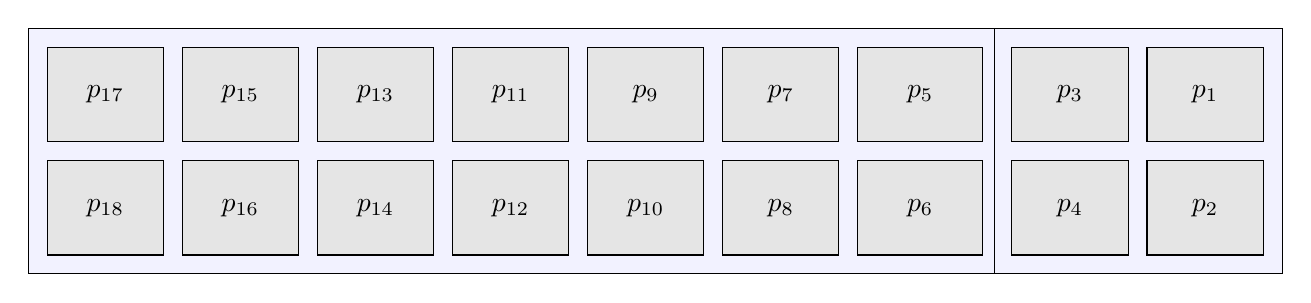
\begin{tikzpicture}[scale=1.2, samples=100]
		
		\filldraw[fill=blue!5!white, draw=black] (0, 0) rectangle (10.23, 2.6);
		
		\filldraw[fill=gray!20!white, draw=black] (0.20, 1.40) rectangle node{$p_{17}$} (1.43, 2.40);
		\filldraw[fill=gray!20!white, draw=black] (0.20, 0.20) rectangle node{$p_{18}$} (1.43, 1.20);
		
		\filldraw[fill=gray!20!white, draw=black] (1.63, 1.40) rectangle node{$p_{15}$} (2.86, 2.40);
		\filldraw[fill=gray!20!white, draw=black] (1.63, 0.20) rectangle node{$p_{16}$} (2.86, 1.20);
		
		\filldraw[fill=gray!20!white, draw=black] (3.06, 1.40) rectangle node{$p_{13}$} (4.29, 2.40);
		\filldraw[fill=gray!20!white, draw=black] (3.06, 0.20) rectangle node{$p_{14}$} (4.29, 1.20);
		
		\filldraw[fill=gray!20!white, draw=black] (4.49, 1.40) rectangle node{$p_{11}$} (5.72, 2.40);
		\filldraw[fill=gray!20!white, draw=black] (4.49, 0.20) rectangle node{$p_{12}$} (5.72, 1.20);
		
		\filldraw[fill=gray!20!white, draw=black] (5.92, 1.40) rectangle node{$p_{9}$} (7.15, 2.40);
		\filldraw[fill=gray!20!white, draw=black] (5.92, 0.20) rectangle node{$p_{10}$} (7.15, 1.20);
		
		\filldraw[fill=gray!20!white, draw=black] (7.35, 1.40) rectangle node{$p_{7}$} (8.58, 2.40);
		\filldraw[fill=gray!20!white, draw=black] (7.35, 0.20) rectangle node{$p_{8}$} (8.58, 1.20);
		
		\filldraw[fill=gray!20!white, draw=black] (8.78, 1.40) rectangle node{$p_{5}$} (10.1, 2.40);
		\filldraw[fill=gray!20!white, draw=black] (8.78, 0.20) rectangle node{$p_{6}$} (10.1, 1.20);
		
		\filldraw[fill=blue!5!white, draw=black] (10.23, 0) rectangle (13.27, 2.6);
		\filldraw[fill=gray!20!white, draw=black] (10.41, 1.40) rectangle node{$p_{3}$} (11.64, 2.40);
		\filldraw[fill=gray!20!white, draw=black] (10.41, 0.20) rectangle node{$p_{4}$} (11.64, 1.20);
		\filldraw[fill=gray!20!white, draw=black] (11.84, 1.40) rectangle node{$p_{1}$} (13.07, 2.40);
		\filldraw[fill=gray!20!white, draw=black] (11.84, 0.20) rectangle node{$p_{2}$} (13.07, 1.20);
		
	\end{tikzpicture}
	
	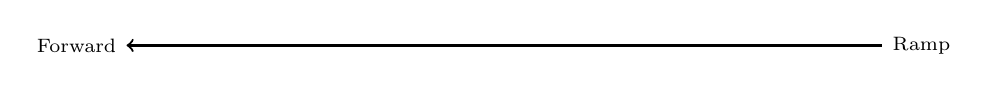
\begin{tikzpicture}[scale=1.2, samples=100]
		\draw[black, thick][<-]  (1, 2.77) node[anchor=east, font=\fontsize{7}{3.5}\selectfont]{Forward} -- (9, 2.77) node[anchor=west, font=\fontsize{7}{3.5}\selectfont]{Ramp} ;
	\end{tikzpicture}
	
	\caption{Aircraft layout} \label{fig:larger}
\end{figure}


The torque applied to the aircraft must keep its CG in the operational range, which corresponds to a fixed percentage of the {\it Mean Aerodynamic Chord} \footnote{Chord is the distance between the leading and trailing edges of the wing, measured parallel to the normal airflow over the wing. The average length of the chord is known as the {\it Mean Aerodynamic Chord} (MAC).} which is considered $1.17m$ for the aircraft of this work. See Figure \ref{fig:lateral}.


\begin{figure}[H]
	\centering
	\includegraphics[scale=0.22]{Images/lateral.png}
	\caption{Aircraft longitudinal cut showing red lines as pallets positions}
	\label{fig:lateral}
\end{figure}

Table \ref{tab:larger} shows the parameters. {\it $D_i^{long}$} and {\it $D_i^{lat}$} refer to the relative distances of pallet centroids (in meters) in relation to the CG of aircraft along both axes.

{\color{blue}

%Note that since the smaller aircraft has a single row of pallets positions, the y-axis passes through the geometric center of each pallet position.  Since the value is 0 for each position, $D_i^{lat}$ is not provided for the smaller aircraft.

Throughout this work, when we refer to the word "torque", we mean item or PC weight x pallet centroid distance to the CG ($D_i^{long}$ or $D_i^{lat}$), considering the angle between these dimensions to always be 90�. In both aircraft, as the ramps have an inclination of 25�, we made the necessary corrections in $D_i^{long}$, {\it Weight} and {\it Volume limits} of the corresponding pallets positions (see Table \ref{tab:larger}).

}


\begin{table}[H]
	\centering
	\caption{Aircraft parameters}  \label{tab:larger}
	\footnotesize
	\begin{tabular}{c | c c c c c c c c c}
		\toprule
		\textbf{Limits}& \multicolumn{3}{c}{$Payload$: 75,000kg} & \multicolumn{3}{c}{$limit^{CG}_{long}$: $1.170m$} &
		\multicolumn{3}{c}{$limit^{CG}_{lat}$: $0.19m$} \\
		\midrule
		\multirow{2}{*}{{\bf Pallets} ($p_i$)}  & $p_{17}$ & $p_{15}$ & $p_{13}$ & $p_{11}$ & $p_{9}$ & $p_{7}$ & $p_{5}$ & $p_{3}$ & $p_{1}$ \\
		& $p_{18}$ & $p_{16}$ & $p_{14}$ & $p_{12}$ & $p_{10}$ & $p_{8}$ & $p_{6}$ & $p_{4}$ & $p_{2}$ \\
		\midrule 
		\multirow{2}{*}{\boldm{$D_i^{long}$} ($m$)} & -17.57 & -13.17 & -8.77 & -4.40 & 0 & 4.40 & 8.77 & 11.47 & 14.89 \\
		& -17.57 & -13.17 & -8.77 & -4.40 & 0 & 4.40 & 8.77 & 11.47 & 14.89 \\			
		\midrule 
		\multirow{2}{*}{\boldm{$D_i^{lat}$} ($m$)}  & 1.32 & 1.32 & 1.32 & 1.32 & 1.32 & 1.32 & 1.32 & 1.32 & 1.32 \\
		& -1.32 & -1.32 & -1.32 & -1.32 & -1.32 & -1.32 & -1.32 & -1.32 & -1.32 \\	
		\midrule
		{\bf Weight limits} ($W_i,\ kg$)      &   4,500   &    4,500  &   4,500   &  4,500    & 4,500     & 4,500     & 4,500     & 4,000    & 3,000   \\
		{\bf Volume limits} ($m^3$)   &   14.8   &   14.8   &  14.8    &  14.8    & 14.8     & 14.8     & 14.8     & 10.0    & 7.0 \\	
		\midrule	
		
		\textbf{Fuel cost rate}  & \multicolumn{9}{c}{ $c_d$ = US\$ $4.900/km$ }	 \\
		
		\midrule
		
		\textbf{Fuel consumption limit rate}  & \multicolumn{9}{c}{ $c_g$ = $5\%$} \\		
		
		\midrule
		
		\textbf{Maximum weight capacity}  & \multicolumn{9}{c}{ $W_{max}$ = $\sum_{i=1}^m W_i$} \\
		
		\bottomrule
	\end{tabular}
	\normalsize 
\end{table}

{\color{blue}
	
The {\it Fuel consumption limit rate} in Table \ref{tab:larger} is the percentage limit of cost increase  due to the CG deviation on the longitudinal axis of the aircraft (this is an arbitrated value for this work that should be better evaluated in future research, as it depends on the characteristics of the aircraft.).

It is important to consider that the range $[0,\ c_g]$ tends to zero as the aircraft attitude tends to level. As the CG deviation varies from 0 to the longitudinal CG limit, the leg cost increase rate varies from 0 to $c_g$.
}

\vspace{3mm}
We also make the following assumptions:
\begin{itemize}
	\item on each pallet, the items are distributed in such a way that their CG coincides with the centroid of the pallet;
	\item the CG of the payload must be at a maximum longitudinal distance of $limit^{CG}_{long}$ from the CG of the aircraft;
	\item the CG of the payload must be at a maximum lateral distance of $limit^{CG}_{lat}$ from the CG of the aircraft;
	\item pallets positions are distributed in two identical rows (with odd and even indices, respectively), and their centroids are at a distance $D^{lat}_{i}$ (where $i$ is the pallet index) from the center-line of the aircraft.
\end{itemize}

\subsection{Problem Summary}

\newcolumntype{M}{>{\raggedright}p{0.03\textwidth}}
\newcolumntype{T}{>{\raggedright\arraybackslash}p{0.9\textwidth}}

\bgroup
\def\arraystretch{1.2}
\begin{table}[H]
	\centering
	\small
	\begin{tabular}{MT}
		&Informally, ACLP+RPDP can be summarised as follows:\\
		\midrule
		max &  (items score sum) / (tour cost) of picked up and delivered items at each node on a tour  \\
		\midrule
s.t.    & Along a tour, the set of unvisited nodes is updated. \\
		& In each node, an item may be included in at most one pallet.\\		
		& In each node, {\it Packed Contents (PC)} are composed of items with the same destination. \\
		& Weight, volume and score of a PC are the corresponding sum of its components.\\
		& A PC remains on board until its destination.\\	
		& Items and a PC can only be included in the same pallet if their destinations are the same.\\
		& Only items destined to the remaining nodes can be loaded.  \\
		& The lateral and longitudinal torques must be within the operational range of the aircraft.\\
		& Weight and volume limitations of the pallets must be respected.\\
		& The total weight must be less than the aircraft payload or the total pallet capacity, whichever is the lowest.\\	
		\midrule
	\end{tabular}
	\normalsize
\end{table}
\egroup 



\section{The mathematical modeling}
\label{sec4}

Given the assumptions, scenarios and parameters described in the previous section, we are ready to present the mathematical modeling of the ACLP+RPDP.

\vspace{3mm}
\textbf{Problem structure and input data:}

Let $C=\{c_{ab}\}$ be the cost matrix of flights, where $c_{ab} = c_d*d(l_a,l_b), 0 \leq a,b \leq \mbox{K}$.

Let $S_K = \{s: \{1, \dots, \mbox{K}\} \rightarrow \{1, \dots, \mbox{K}\} \}$ be the set of $\mbox{K}!$ permutations indexed by $\pi$, which correspond to all possible tours (or itineraries) that have node $0$ as origin and end, passing through the other $\mbox{K}$ nodes.

Note that $\pi_k$ is the node in position $k$ of tour $\pi$, and $\pi_0$ is always node 0, the base.

$\tau^{\pi_k}$ is the total torque applied by the loaded pallets to the aircraft in this node. 
	
Let $L = \{ 0, \pi_1, \ldots, \pi_{K} \}$ be a tour with $\mbox{K}+1$ nodes.

Let $d(\pi_a,\ \pi_b)$ be the distance from $\pi_a$ to $\pi_b$, where $0 \leq a,\ b \leq \mbox{K}$. By definition, $d(\pi_a,\ \pi_a)\ =\ 0$.

Let $L^{\pi_k}$ be the set of remaining nodes when the aircraft is in $\pi_k$, $0 \leq k \leq \mbox{K}$. Therefore, $L^{\pi_0}\ =\ L$ and $L^{\pi_K}\ =\ \{ 0 \}$.

Let $M^{\pi_k} = \{1, 2, \ldots, m \}$ the set of $m$ empty pallets assigned to specific positions within an aircraft. Each pallet $i$, has weight capacity $W_i$, volume capacity $V_i$, pallet destinations $to^{\pi_k}_i$, $0 \leq k \leq K$, the longitudinal distance to the CG of aircraft $D^{long}_i$, and the lateral distance to the center line of aircraft $D^{lat}_i$. Note that all pallets and aircraft attributes are in uppercase.

Let $N^{\pi_k} = \{1, 2, \ldots, n^{\pi_k} \}$ be the set of $n^{\pi_k}$ items $t_j^{{\pi_k}}$ existent in node $\pi_k$, $0 \leq k \leq K$. Each item $j$, has score $s_j$, weight $w_j$, volume $v_j$, and destination $to_j \in L^{\pi_k}$. Let $N = \bigcup_{0 \leq k \leq K} N^{\pi_k}$ be the set of items of all nodes along a tour.

Let $Q^{\pi_k} = \{1, 2, \ldots, m^{\pi_k} \}$ be the set of packed contents (PC) in $m^{\pi_k} \leq m$ pallets that will remain on board when the aircraft arrives at node $\pi_k$, with $0 \leq k \leq K$. $a^{\pi_k}_q$, $1 \leq q \leq m^{\pi_k}$, is the set of picked-up items that were allocated on a pallet in some of the previous nodes. Note that $Q^0 = \{\ \}$ as there is no PC departing from the base.

Note that all items and PC attributes are in lowercase.

$a^{\pi_k}_q$ has total weight $w_q$, total volume $v_q$, and destination $to_q^{\pi_k} \in L^{\pi_k} \cup \{\pi_k\}$. If $to_q^{\pi_k} = \pi_k$, then $a^{\pi_k}_q$ is unloaded, and the pallet will be available to receive other packet items; otherwise, $a^{\pi_k}_q$ remains on the aircraft, eventually in another pallet, and with some items of $N^{\pi_k}$ having the same destination.


\vspace{3mm}
\textbf{The decision variables:}

Let $X_{ij}^{\pi_k}$ and $Y_{iq}^{\pi_k}$ be binary variables, where $0 \leq k \leq \mbox{K}$, $1 \leq j \leq n^{\pi_k}$, $1 \leq i \leq m$ and $1 \leq q \leq m^{\pi_k}$.

$X_{ij}^{\pi_k} = 1$ if item $t_j^{{\pi_k}}$ is assigned to pallet $i$ in node $\pi_k$, and 0 otherwise.

$Y_{iq}^{\pi_k} = 1$ if a PC $a_q^{{\pi_k}}$ is assigned to pallet $i$ in node $\pi_k$, and 0 otherwise. By definition, $Y_{iq}^0=0$.


\vspace{3mm}
\textbf{The structure of a solution:}

Allocations of items or PC to pallets position in the node $\pi_k$ can be seen as a bipartite graph $G^{\pi_k}(V^{\pi_k}, E^{\pi_k})$,
where:

$V^{\pi_k} = M^{\pi_k} \cup N^{\pi_k} \cup Q^{\pi_k}$,

$E^{\pi_k} = E^M_{N^{\pi_k}} \cup E^M_{Q^{\pi_k}}$,

$(i, j) \in E^M_{N^{\pi_k}}$ if $X_{ij}^{\pi_k} = 1$, and

$(i, q) \in E^M_{Q^{\pi_k}}$ if $Y_{iq}^{\pi_k} = 1$.

\vspace{3mm}
\textbf{The objective function:}

The objective of ACLP+RPDP is to find the permutation $\pi \in S_K$, with the corresponding allocation of items on the pallets at each node, that maximizes the function $\tilde{s}_\pi/\tilde{c}_\pi$ \ref{eq1}, where $\tilde{s}_\pi$\/ is the total score of transported items, and  $\tilde{c}_\pi$\/ is the total cost of fuel consumed. In this way, the tour is described as $\{0,\ {\pi(1)},\ \ldots,\ {\pi(K)},\ 0\}$.

\begin{equation} \label{eq1}
	\max_{\pi \in S_K} \tilde{s}_\pi/\tilde{c}_\pi
\end{equation}

\vspace{3mm}
\textbf{Where:}
\vspace{3mm}

\begin{equation} \label{eq:scores}
	\tilde{s}_\pi = \sum_{k=0}^{K} \sum_{i=1}^{m} \sum_{j=1}^{n^{\pi_k}} X_{ij}^{\pi_k} \times s_j
\end{equation}

\vspace{3mm}
In Equation \ref{eq:tau}, $\tau^{\pi_k}$ is the total torque applied to the aircraft in node ${\pi_k}$. This is the sum of all pallets torque (pallet centroid distance to the CG times the total weight packed on the pallet).

\begin{equation} \label{eq:tau}
	\tau^{\pi_k} = \sum_{i=1}^{m} \Big [ D_i^{long} \times (\sum_{j=1}^{n^{\pi_k}} X_{ij}^{\pi_k} \times w_j +  \sum_{q=1}^{m^{\pi_k}} Y_{iq}^{\pi_k} \times w_q) \Big ];\ k \in \{0,1,2, \ldots, \mbox{K}\}
\end{equation}

\vspace{3mm}
In Equation \ref{eq:eps}, $\epsilon^{\pi_k}$ the torque applied to the aircraft in node ${\pi_k}$ divided by the maximum torque possible.

\begin{equation} \label{eq:eps}
	\epsilon^{\pi_k} = \frac{\tau^{\pi_k}}{W_{max} \times limit^{CG}_{long}};\ k \in \{0,1,2, \ldots, \mbox{K}\}
\end{equation}

\vspace{3mm}
In the tour cost calculation in Equation \ref{eq:costs}, the first parcel denotes the fuel cost from the base until the last node, and the second the fuel cost in the last leg, from the last node back to the base.

\begin{equation} \label{eq:costs}
	\tilde{c} = \sum_{k=0}^{K-1} \Big [ c^{\pi_k, \pi(k+1)}\times(1+c_g\times|\epsilon^{\pi_k}|) \Big ] + c^{\pi_K,0}\times(1+c_g\times|\epsilon^{\pi_K}|)
\end{equation}

\vspace{3mm}
Equations \ref{eq:pdp11} and \ref{eq:departing} state the set of unvisited nodes departing from the base ($0$) and $\pi_k$.

\begin{equation} \label{eq:pdp11}
	L^{0} = L
\end{equation}

\begin{equation} \label{eq:departing}
	L^{\pi_k} = L^{\pi_{k-1}} - \{\pi_k\}; \ k \in \{1,2, \ldots, \mbox{K}\}
\end{equation}

	
\vspace{3mm}	
Although there are no items packed at the beginning of the transportation plan, we defined these variables for ease of notation \ref{eq:pdp13}. 
	
\begin{equation} \label{eq:pdp13}
	Y^0_{iq} = 0; w_q^0 = 0; v_q^0 = 0; to_q^0 = -1;\ i,q \in \{1, 2, \ldots, m\}
\end{equation}

\vspace{3mm}
PC appear when there are items on the pallets that will not be unloaded on the next node.
The PC's total weight (\ref{eq:cons2}) and volume (\ref{eq:cons3}) correspond to all the items that were on the pallet, since all these items have the same destination.

\begin{equation} \label{eq:cons2}
	w_q^{\pi(k+1)} = \sum_{j=1}^{n^{\pi_k}} X_{ij}^{\pi_k} \times w_j + \sum_{q=1}^{m^{\pi_k}} Y_{iq}^{\pi_k} \times w_q;  \ q \in \{1, 2, \ldots, m^{\pi_k}\}; k \in \{0,1,2, \ldots, \mbox{K-1}\}
\end{equation}

\begin{equation} \label{eq:cons3}
	v_q^{\pi(k+1)} = \sum_{j=1}^{n^{\pi_k}} X_{ij}^{\pi_k} \times v_j + \sum_{q=1}^{m^{\pi_k}} Y_{iq}^{\pi_k} \times v_q;  \ q \in \{1, 2, \ldots, m^{\pi_k}\}; k \in \{0,1,2, \ldots, \mbox{K-1}\}
\end{equation}

\vspace{3mm}
Equations \ref{eq:LatItem} and \ref{eq:LatPacked} calculate the weight differences between the aircraft sides to be used ahead in the constraint of the CG lateral deviation through Equation \ref{eq:torqlat}.

\begin{equation} \label{eq:LatItem}
	w^{\pi_k}_{items}   = \sum_{i=1}^{m} \sum_{j=1}^{n^{\pi_k}}  \Big ( X_{ij}^{\pi_k} \times w_j \times (i\%2) - X_{ij}^{\pi_k} \times w_j \times (i+1)\%2 \Big ); \ k \in \{0,1,2, \ldots, \mbox{K}\}
\end{equation}

\begin{equation} \label{eq:LatPacked}
	w^{\pi_k}_{packed} =  \sum_{i=1}^{m} \sum_{q=1}^{m^{\pi_k}} \Big ( Y_{iq}^{\pi_k} \times w_q \times (i\%2) - Y_{iq}^{\pi_k} \times w_q \times (i+1)\%2 \Big ); \ k \in \{0,1,2, \ldots, \mbox{K}\}
\end{equation}

\vspace{3mm}
\textbf{Subject to:}
\vspace{3mm}

Load only items and keep boarded PC destined to the unvisited nodes (\ref{eq:pdp12} and \ref{eq:pdp9}).

\begin{equation} \label{eq:pdp12}
	X_{ij}^{\pi_k} = 0;\ to_j \notin L^{\pi_k}; \ i \in \{1, 2, \ldots, m\}; \ j \in \{1, 2, \ldots, n^{\pi_k}\}; \ k \in \{0,1,2, \ldots, \mbox{K}\}
\end{equation}

\begin{equation} \label{eq:pdp9}
	Y_{iq}^{\pi_k} = 0;\ to_q \notin L^{\pi_k}; \ i \in \{1, 2, \ldots, m\}; \ q \in \{1, 2, \ldots, m^{\pi_k}; \ k \in \{0,1,2, \ldots, \mbox{K}\}
\end{equation}


\vspace{3mm}
The Equation \ref{eq:torqlat} is the lateral torque constraint for the aircraft, while the Equation \ref{eq:torqlong} is the longitudinal torque constraint.

\begin{equation} \label{eq:torqlat}
	D_i^{lat} \times \Big | w^{\pi_k}_{items} + w^{\pi_k}_{packed} \Big | \leq  W_{max} \times limit^{CG}_{lat}; \ k \in \{0,1,2, \ldots, \mbox{K}\}
\end{equation}

\begin{equation} \label{eq:torqlong}
	\Big | \tau^{\pi_k} \Big | \leq W_{max} \times limit^{CG}_{long};\ k \in \{0,1,2, \ldots, \mbox{K}\}
\end{equation}

\vspace{3mm}
The weight limitation of the aircraft must be respected \ref{eq:payload}. The sum of weights \ref{eq:app2} and volumes \ref{eq:app3} in each pallet must not exceed its capacity. Each item is associated with a pallet at most \ref{eq:app4}.

\begin{equation} \label{eq:payload}
	\sum_{i=1}^{m^{\pi_k}} \Big (\sum_{j=1}^{n^{\pi_k}} X_{ij}^{\pi_k} \times w_j + \sum_{q=1}^{m^{\pi_k}} Y_{iq}^{\pi_k} \times w_q \Big ) \leq W_{max}; \ k \in \{0,1,2, \ldots, \mbox{K}\}
\end{equation}

\begin{equation} \label{eq:app2}
	\sum_{j=1}^{n^{\pi_k}} X_{ij}^{\pi_k} \times w_j + \sum_{q=1}^{m^{\pi_k}} Y_{iq}^{\pi_k} \times w_q  \leq W_i; \ i \in \{1, 2, \ldots, m\}; \ k \in \{0,1,2, \ldots, \mbox{K}\}
\end{equation}

\begin{equation} \label{eq:app3}
	\sum_{j=1}^{n^{\pi_k}} X_{ij}^{\pi_k} \times v_j + \sum_{q=1}^{m^{\pi_k}} Y_{iq}^{\pi_k} \times v_q  \leq\ V_i; \ i \in \{1, 2, \ldots, m\}; \ k \in \{0,1,2, \ldots, \mbox{K}\}
\end{equation}

\begin{equation} \label{eq:app4}
	\sum_{i=1}^{m} X_{ij}^{\pi_k} \leq 1; \ j \in \{1, 2, \ldots, n^{\pi_k}\}; \ k \in \{0,1,2, \ldots, \mbox{K}\}
\end{equation}


\vspace{3mm}
Equations \ref{eq18} and \ref{eq19} were set to group items with the same destinations. 

\begin{equation} \label{eq18}
	to_a - to_b \geq -K \times (1-X_{ia}^{\pi_k} \times X_{ib}^{\pi_k}); \ a,b \in \{1, 2, \ldots, n^{\pi_k}\}; \ k \in \{0, 1, \ldots, K\}
\end{equation}

\begin{equation} \label{eq19}
	to_a - to_b \leq K \times (1-X_{ia}^{\pi_k} \times X_{ib}^{\pi_k}); \ a,b \in \{1, 2, \ldots, n^{\pi_k}\}; \ k \in \{0, 1, \ldots, K\}
\end{equation}

\vspace{3mm}
A PC is allocated to a pallet if its destination in in the not visited nodes set.
\begin{equation} \label{eq17}
	Y_{iq}^{\pi_k} = 1; \ q \in \{1, 2, \ldots, m^{\pi_k}\}; \ k \in \{1, \ldots, K\};  \ to_q \in L^{\pi_k}
\end{equation}

\vspace{3mm}
Equations \ref{eq20} and \ref{eq21} were set to group items and PC with the same destinations. 

\begin{equation} \label{eq20}
	to_j - to_q \geq -K \times (1-X_{ij}^{\pi_k} \times Y_{iq}^k); \ j \in \{1, 2, \ldots, n^{\pi_k}\}; \ q \in \{1, 2, \ldots, m^{\pi_k}\}; \ k \in \{0, 1, \ldots, K\}
\end{equation}

\begin{equation} \label{eq21}
	to_j - to_q \leq  K \times (1-X_{ij}^{\pi_k} \times Y_{iq}^k); \ j \in \{1, 2, \ldots, n^{\pi_k}\}; \ q \in \{1, 2, \ldots, m^{\pi_k}\}; \ k \in \{0, 1, \ldots, K\}
\end{equation}


\vspace{3mm}
The PC must remain on board \ref{eq:app5} until their destinations. 

\begin{equation} \label{eq:app5}
	Y_{iq}^{\pi_k} = 1;\ to_q \in L^{\pi_k}; \ q \in \{1, 2, \ldots, m^{\pi_k}\}; \ k \in \{0,1,2, \ldots, \mbox{K}\}
\end{equation}


Until this point, our research problem has been thoroughly described, and it is certainly very difficult since it combines several sub-problems, which are difficult to solve in their own right. Then, we develop an innovative process to efficiently solve it.


\section{Solution strategy}
\label{sec5}

Once the assumptions of this work and the mathematical modeling of the problem are presented, it is easy to see that ACLP+RPDP is NP-hard. In a similar way to Lurkin and Schyns \cite[p. 6]{LurkinSchyns2015}, consider the simple case where $K=1$\/ (one leg), $m=2$ (two pallets around the aircraft CG), $2n$\/ sufficiently light items with same scores in node 0, and no items in node 1. Under these conditions, through polynomial reductions for the {\it Set-Partition Problem}, it is possible to demonstrate that the decision problem associated with ACLP+RPDP is NP-complete.

{\color{blue}

Equations \ref{eq18} and \ref{eq19} were set to group items with the same destinations. But, as they mean a combination of $n^{\pi_k}$ items 2 by 2, this may easily lead to huge numbers, 60,000 to 320,000 possible combinations, due to the number of items in each node, which together with the other constraints make a MIP solution very hard.

To work around this, we decided to create the destination attribute for the pallets ($TO_i^{\pi_k}$), to reduce the number of combinations and enable the solution using heuristics.  $TO^{\pi_k}_i$ denotes that pallet $i$ may assume a different destination in each node ${\pi_k}$.

On subsequent nodes, the PC can be allocated with other items of same destination \ref{eq:cons5}.

\begin{equation} \label{eq:cons5}
	TO_i^{\pi(k+1)} = to_j;\ X^{\pi_k}_{ij} = 1  \ \mbox{and}\ to_j \in L^{\pi_{k+1}};  \ i \in \{1, 2, \ldots, m\}; \ j \in \{1, 2, \ldots, n^{\pi_k}\}; \ k \in \{0,1,2, \ldots, \mbox{K-1}\}
\end{equation}

\vspace{3mm}
At each node, an item (\ref{eq:pdp8}) and the already packed contents (\ref{eq:pdp2}) must only be allocated to a pallet if the destinations are the same.

\begin{equation} \label{eq:pdp8}
	TO_i^{\pi_k} = to_j;\ X_{ij}^{\pi_k} = 1; \ i \in \{1, 2, \ldots, m\}; \ j \in \{1, 2, \ldots, n^{\pi_k}\}; \ k \in \{0,1,2, \ldots, \mbox{K}\}
\end{equation}

\begin{equation} \label{eq:pdp2}
	TO_i^{\pi_k} = to_q;\ Y_{iq}^{\pi_k} = 1; \ i \in \{1, 2, \ldots, m\};\ q \in \{1, 2, \ldots, m^{\pi_k}\}; \ k \in \{0,1,2, \ldots, \mbox{K}\}
\end{equation}

}

Real cases are more complex as they have hundreds of different items in each node and involve four intractable sub-problems: APP, WBP, PDP and TSP. Through the mathematical modeling presented in the previous section, we verify that {\it Mixed-Integer Programming}\/ (MIP) is not able to solve these cases in feasible time. Thus, it is necessary to adopt some strategy to find a viable solution, not necessarily optimal, that seeks to maximize the objective function $f_{\pi}$.

Our strategy is based on the fact that, in real cases, $K$\/ is usually small. Specifically, we will consider $K \leq 6$\/ throughout this work, which is a higher value than usual in {\it Brazilian Air Force}'s missions. As a result, if we have fast node-by-node solutions that allow us to construct a complete tour, we will be able to test all possible $K!$\/ tours and thus select the one that provides the best value for the $f_{\pi}$\/ function.

{\color{blue}Another possibility to make this approach more general is to devise some bounding schemes to allow discarding most higher-cost tours and allowing an increase in the number of nodes without compromising performance.}

For now, our tactic will be, at each shipping node, to predefine the destinations of the pallets at that node. In this way, we will reserve a number of pallets proportional to the volume demanded by each destination at the shipping node (we could have used another criterion, but it was observed in the experiments that volume is more constrictive in airlift).
Once the destinations of the pallets are defined, we will use heuristics and a MIP solver to find the best possible node-by-node solution. This strategy is summarized in Algorithm \ref{alg:main}.


\begin{algorithm}[H]
	\caption{Solves ACLP+RPDP for a scenario with certain volume surplus (1.2, 1.5, or 2.0)}  \label{alg:main}
	\begin{algorithmic}[1]
		
		\Procedure{$ACLP+RPDP$}{$scenario,\ surplus,\ timeLim$}
		
		\State Let $L, M, C$ be according to $scenario$ \label{main:LMC} \Comment{Nodes, pallets and costs}
		
		\State $N \gets ItemsGeneration(scenario,\ volume)$ \label{main:items} \Comment{Items available for shipment}
		
		\For {each $method$} \Comment{$method$ is a MIP solver or a heuristic}
			\For {each $\pi \in S_K$} \label{main:loop1} \Comment{$\pi$ is a permutation of nodes (a tour)}
				\State $f_{\pi} \gets SolveTour(\pi, L, M, C, N, method,\ timeLim )$ \Comment{a solution to the tour $\pi$} \label{main:method}
			\EndFor \label{main:loop2}
			\State $answer[scenario,surplus,method] \gets \max f_{\pi}$ \label{main:f} \Comment{Best result among all permutations}
		\EndFor
		
		\Return $answer$
		
		\EndProcedure
		
	\end{algorithmic}
\end{algorithm}

{\color{blue}
	Until scenario 4, solving all tours and selecting the best is fast enough for operational use. For scenarios 4 and 5 (which are not typical in the Brazilian Air Force), we plan bounding schemes to allow for the discarding of most of the higher-cost tours. This is expected to reduce the running time for scenarios 4 and 5, favoring the discovery of better search mechanisms as well as further applications that may require more nodes per tour.	
}

In this algorithm, there are six values for the $scenario$\/ parameter, according to Table \ref{tab:scenarios}, which defines $K$, the sets of nodes, the aircraft, the pallets and the costs from Tables \ref{tab:smaller} or \ref{tab:larger} that will be used (line \ref{main:LMC}).

The parameter $volume$\/ is a value in (1.2, 1.5, 2.0), which corresponds, at each node $\pi_k$, to the ratio between the sum of the volumes of the items ($\sum_{j=1}^{n^{\pi_k}} v_j$) and the load capacity of the pallets ($\sum_{i=1}^{m} V_i$). This parameter is passed to $ItemsGeneration$\/ (line \ref{main:items}), responsible for creating the items to be shipped, which will be presented in the next section (Algorithm \ref{alg:itemsgen}).

The parameter $method$\/ corresponds to a MIP solver or a heuristic that we will present in subsection \ref{methods}. The loop of lines \ref{main:loop1}-\ref{main:loop2} goes through all permutations, where the node-by-node solutions are performed by $SolveTour$, whose result is stored in $f_{\pi}$. The best result among all $K!$\/ tours will be the answer for $scenario$, $volume$\/ and $method$\/ (line \ref{main:f}).


\vspace{2.0mm}
\begin{table}[H]
	\centering
	\caption{Testing scenarios}  \label{tab:scenarios}
	\begin{tabular}{c c c }
		\toprule
		{\bf Scenario} & {$K$} & {$L^{0}$} \\		
		\midrule
		1 & 2    & \{$\pi_1,\ \pi_2,\ 0$\}                                 \\
		2 & 3    & \{$\pi_1,\ \pi_2,\ \pi_3,\ 0$\}                         \\
		3 & 4    & \{$\pi_1,\ \pi_2,\ \pi_3,\ \pi_4,\ 0$\}                 \\
		4 & 5    & \{$\pi_1,\ \pi_2,\ \pi_3,\ \pi_4,\ \pi_5,\ 0$\}         \\
		5 & 6    & \{$\pi_1,\ \pi_2,\ \pi_3,\ \pi_4,\ \pi_5,\ \pi_6,\ 0$\} \\
		\bottomrule
	\end{tabular}
\end{table}

{\color{blue} Column $L^{0}$ in Table \ref{tab:scenarios} represents the set of non-visited nodes staying in the base. }

Next, we will present two subsections: in the first we explain how $SolveTour$ is executed, while in the second we will present the heuristic developed for node-by-node resolutions.


\subsection{SolveTour algorithm}
\label{tour}

In addition to the set of nodes, pallets, costs and items, $SolveTour$, described in Algorithm \ref{alg:tour}, receives the parameter $method$, which corresponds to a MIP solver or a heuristic for solving the node-by-node problems, and the parameter $\pi$, which is a {\color{blue} permutation of nodes (excluding the base)} that defines the order of visits in this tour.

As we mentioned in the previous section, all tours start and end at the base\/ (lines \ref{tour:pi1}-\ref{tour:pi2}). After initializing the score and cost values (lines \ref{tour:score}-\ref{tour:cost}), there is a loop for the $K+1$\/ flights (lines \ref{tour:loop1}-\ref{tour:loop2}). Initially we set pallets destination as $\mbox{-1}$\/ (line \ref{tour:-1}).

When the aircraft is at the base, the initial graph $G_1$\/ is empty because it has no PC \ref{tour:g11}. Otherwise, the set $L^{\pi_k}$\/ of remaining nodes is updated (line \ref{tour:lk1}), and $UpdatePacked$\/ (line \ref{tour:dest}) returns the set of PC that have not yet reached their destination and remain on board, rearranging them on the pallets to minimize CG deviation. This allocation is stored in graph $G_1$\/ (line \ref{tour:g12}).

In the context of this work, we know that $m>K$, once the aircraft has $18$\/ pallets {\color{blue}} and $K\leq6$, allowing there to be at least one pallet for each node to be visited. $SetPalletsDestinations$\/ (line \ref{tour:dest2}) presets the destination of each pallet based on the volume demands of the current node, without changing the pallets destination with PC (packed contents).

Finally, $SolveNode$\/ includes the edges corresponding to the items shipped at the current node, returning the graph $G_2$\/ (line \ref{tour:node}). The score and the CG deviation of this graph are calculated (line \ref{tour:analyse}) and accumulated (lines \ref{tour:score2}-\ref{tour:cost2}), allowing the final result of this tour (line \ref{tour:f}).

\begin{algorithm}[H]
	\caption{Procedure to solve tour $\pi$ with $method$ (MIP solver or heuristic)}  \label{alg:tour}
	\begin{algorithmic}[1]
		
		\Procedure{$SolveTour$}{$\pi, L, M, C, N, method$}
		
		\State $\pi_0     \gets 0$ \label{tour:pi1} \Comment{The first node is the base}
		\State $\pi_{K+1} \gets 0$ \label{tour:pi2} \Comment{The last node is also the base}

		\State $score \gets 0$ \label{tour:score}
		\State $cost  \gets 0$ \label{tour:cost}
		
		\For {$k \in \{0,1,2,...,K\}$} \label{tour:loop1}	
			
			\For{$i \in \{1,2,3,...,m\}$}
				\State $to_i^{\pi_k} \gets -1$ \label{tour:-1} \Comment{unset the pallet destination}
			\EndFor	
			
			\If {$k = 0$}
				\State $L^0 \gets L - \{0\}$
				\State Let $G_1(M \cup N^0, \varnothing)$ \label{tour:g11}
			\Else
				\State $L^{\pi_k} \gets L - \{0,...,\pi_k\}$  \label{tour:lk1}	\Comment{$\pi_k$ is the current node}		
				\State $E^M_{Q^{\pi_k}}, M \gets UpdatePacked(M, Q^{\pi_k}, \pi_k)$ \label{tour:dest}			
				\State Let $G_1(M \cup N^{\pi_k} \cup Q^{\pi_k}, E^M_{Q^{\pi_k}})$ \label{tour:g12}
			\EndIf  \label{tour:lk2}	
			
			\State $M \gets SetPalletsDestinations(M, \pi_k )$ \label{tour:dest2}
					
			\State $G_2 \gets SolveNode(method, \pi_k, G_1)$ \label{tour:node}
			
			\State $s, \epsilon \gets ScoreAndDeviation(\pi_k, G_2)$ \label{tour:analyse}
			
			\State $score \gets score + s$ \label{tour:score2}
			\State $cost  \gets cost  + c_{\pi_k,\pi_{k+1}} \times (1 + c_g \times |\epsilon|)$ \label{tour:cost2} 
		
		\EndFor  \label{tour:loop2}
		
		\Return $score / cost$ \label{tour:f}
		
		\EndProcedure
		
	\end{algorithmic}
\end{algorithm}

{\color{blue}

$UpdatePacked$, described in Algorithm \ref{alg:cons}, finds the best packet-pallet allocation, in terms of CG deviation, for the PC that remain on board.
Then $MinCGDeviation$\/ (line \ref{cons:minCG}) is run through a MIP solver ({\it Gurobi}) with the equations \ref{eq:torque}, \ref{eq:embarked} and \ref {eq:one}, to relocate the PC on the pallets, minimizing torque and ensuring that they all remain on board, one PC on each pallet.
As there are few variables, the MIP solver returns an allocation $E^M_{Q^{\pi_k}}$ in less than 30 milliseconds.
Finally, the destination of each pallet with a PC is updated (lines \ref{cons:Ybegin}-\ref{cons:Yend}).

}

\begin{algorithm}[H]
	\caption{Procedure to update the PC that remain boarded on node $\pi_k$}  \label{alg:cons}
	\begin{algorithmic}[1]
		
		\Procedure{$UpdatePacked$}{${M, Q^{\pi_k}, \pi_k}$}
						
		\State $E^M_{Q^{\pi_k}} \gets MinCGDeviation(E^M_{Q^{\pi_k}})$ \label{cons:minCG}
		
		\For{$i \in \{ 1, 2, \ldots, m \}$} \label{cons:Ybegin}
		
			\For{$q  \in \{ 1, 2, \ldots, m^{\pi_k} \}$}
			
				\State $to_i^{\pi_k} \gets -1$
			
				\If{$(i, q) \in E^M_{Q^{\pi_k}}$} 
					\State $to_i^{\pi_k} \gets to_q$   \Comment{set the pallet destination.}
				\EndIf
			\EndFor		
		\EndFor \label{cons:Yend}
		
		\Return $E^M_{Q^{\pi_k}}, M$
		
		\EndProcedure
		
	\end{algorithmic}
\end{algorithm}

\vspace{3mm}
$MinCGDeviation$ objective function:

\begin{equation} \label{eq:torque}
	\mbox{minimize}\ \Big | \sum_{i=1}^{m} \sum_{q=1}^{m^{\pi_k}} Y^k_{iq} \times w_q \times D_i^{long}  \Big |
\end{equation}

\vspace{3mm}
s.t.:

\begin{equation} \label{eq:embarked}
	\sum_{i=1}^{m} Y^k_{iq} = 1;\ q \in \{1,2,\ldots,m^{\pi_k}\}
\end{equation}

\begin{equation} \label{eq:one}
	\sum_{q=1}^{m^{\pi_k}} Y^k_{iq} \leq 1;\ i \in \{1,2,\ldots,m\}
\end{equation}


$SetPalletsDestinations$, {\color{blue}which sets pallets' destinations not yet defined}, is described in Algorithm \ref{alg:dest}.

The set $volumes$ stores the demand volume of items destined to the non-visited nodes ($L^{\pi_k}$) (line \ref{dest:vector1}).

The destinations of each pallet are defined proportionally to the volume of items, regarding the pallets with a PC (lines \ref{dest:propor1}-\ref{dest:propor2}).

The node with the maximum volume demand defines the destination of any remaining pallets (lines \ref{dest:max1}-\ref{dest:max2}).


\begin{algorithm}[H]
	\caption{Procedure to set pallets destinations based on the items to be embarked on node $k$}  \label{alg:dest}
	\begin{algorithmic}[1]
		
		\Procedure{$SetPalletsDestinations$}{$M, \pi_k$}
				
			\State $volumes \gets \{ 0\ |\ L^{\pi_k} \}$  \label{dest:vector1}

			\State $max \gets 0$ \label{dest:max} \Comment{destination with maximum volume demand.}
	
			\State $total \gets 0$ 
	
			\For{$j \in \{ 1,2,3,...,n^{\pi_k} \}$}
						
				\If {$to_j \in L^{\pi_k}$} 
				
					\State $volumes_{to_j} \gets volumes_{to_j} + v_j$ 
					\State $total \gets total + v_j$ 
					
					\If {$volumes_{to_j} > volumes_{max}$}
					
						\State $max \gets to_j$ 
					\EndIf
					
				\EndIf
				
			\EndFor
					
			\For{$x \in L^{\pi_k}$} \label{dest:propor1}
			
				\If {$volumes^{x} \neq 0$}
				
					\State $needed \gets \max \{1, \lfloor{ m \times volumes_{x}/total}\rfloor \}$  \Comment{number of pallets needed}
					
					\State $np \gets 0$
					
					\For{$i \in \{1,2,3,...,m\}$}
											
						\If{$np < needed$ {\bf and} $to_i^{\pi_k} = -1$}              \Comment{if the pallet destination in node $k$ is unset}
							\State $to_i^{\pi_k} \gets x$
							\State $np \gets np + 1$
						\EndIf
					
					\EndFor
				\EndIf 
				
			\EndFor \label{dest:propor2}
		
			\For{$i \in \{1,2,3,...,m\}$} \label{dest:max1}
				\If{$to_i^{\pi_k} \gets -1$}
					\State $to_i^{\pi_k} \gets max$
				\EndIf
			\EndFor \label{dest:max2}
			
			\Return $M$
			
		\EndProcedure
		
	\end{algorithmic}
\end{algorithm}


$ScoreAndDeviation$\/ is described in Algorithm \ref{alg:eval}, which evaluates the allocation graph generated by $SolveNode$, returning the corresponding score and CG deviation. It consists of a loop that goes through all the pallets (lines \ref{eval:loop1}-\ref{eval:loop2}), accumulating the scores (lines \ref{eval:score1}-\ref{eval:score2} ) and the torques (lines \ref{eval:eps1}-\ref{eval:eps2}) of the shipped items, allowing the final calculation of the CG deviation (lines \ref{eval:torque1}-\ref{eval:torque2}).


\begin{algorithm}[H]
	\caption{Procedure to calculate the solution score and the relative torque deviation in node $\pi_k$}  \label{alg:eval}
	\begin{algorithmic}[1]
		
		\Procedure{$ScoreAndDeviation$}{$\pi_k,\ G$}
		
		\State Let $G(M \cup N^{\pi_k} \cup Q^{\pi_k}, E^M_{Q^{\pi_k}} \cup E^M_{N^{\pi_k}})$
		
		\State Let $X_{ij}^{\pi_k} = 1$ if $(i, j) \in E^M_{N^{\pi_k}}$, $1 \leq i \leq m$, $1 \leq j \leq n^{\pi_k}$
		\State Let $Y_{iq}^{\pi_k} = 1$ if $(i, q) \in E^M_{Q^{\pi_k}}$, $1 \leq i \leq m$, $1 \leq q \leq m^{\pi_k}$
		
		\State $s \gets 0$
		\State $\tau_i \gets \{\ 0\ |\ [1,2,3,...,m]\}$
		
		\For{$i \in \{1,2,3,...,m\}$}	\label{eval:loop1}
						
			\For{$j \in \{1,2,3,...,n^{\pi_k}\}$}
			
				\If{$X_{ij}^{\pi_k} = 1$}
					\State $s \gets s + s_j$ \label{eval:score1}
					\State $\tau_i \gets \tau_i + w_j \times D_i^{long}$ \label{eval:eps1}
				\EndIf
			\EndFor	
					
			\For{$q \in \{1,2,3,...,m^{\pi_k}\}$}
				\If{$Y_{iq}^{\pi_k} = 1$}
					\State $s \gets s + s_q$   \label{eval:score2}
					\State $\tau_i \gets \tau_i + w_q \times D_i^{long}$  \label{eval:eps2}
				\EndIf
			\EndFor	   \label{eval:loop2}
		\EndFor
		
		\State $W_{max} \gets \min(Payload,\ \sum_{1}^{m} W_i)$ \label{eval:torque1}
		
		\State $\tau_{max} \gets W_{max} \times limit^{CG}_{long}$
		
		\State $\epsilon \gets  \sum_{1}^{m} \tau_i / \tau_{max}$ \label{eval:torque2}
		
		\Return $s,\ \epsilon$
		\EndProcedure
		
	\end{algorithmic}
\end{algorithm}


\subsection{Node-by-node solutions}
\label{methods}


In this subsection we present two implementations of $SolveNode(method,\ \pi_k,\ G)$, where  $\pi_k$\/ is the current node and $G$\/ is the allocation graph of the PC that remain on board at node $\pi_k$. These implementations correspond to the two possible values of the $method$\/ parameter: $MIP$\/ ({\it Gurobi}) or $Shims$\/ (a heuristic).


\subsubsection{MIP solver}
\label{solver}

To find a viable solution for ACLP+RPDP, the strategy adopted in $SolveTour$\/ previously defines the values of some variables. Concretely, all permutations between the nodes are tested, the set of nodes to be visited is updated, the PC that remain on board are reallocated to minimize the CG deviation, and the pallets destination is determined according to the volume of items available for shipment. In this way, the mathematical modeling for $SolveNode(MIP,\ \pi_k,\ G)$\/ becomes simpler, which finds an allocation of available items in node $\pi_k$\/ using previously defined values of $L^{\pi_k}$, $to_i^{\pi_k}$, and $a^{\pi_k}_q$. 

This simplified modeling is described in the equations \ref{eq:obj2} to \ref{eq:if2}, which maximizes the score of the $n^{\pi_k}$ items to be shipped, maintaining load balancing.

The variables $X_{ij}$ and $Y_{iq}$ define the sets of edges $E^M_{N^{\pi_k}}$ and $E^M_{Q^{\pi_k}}$, respectively, which will be added to the graph $G$.

\vspace{3mm}
\textbf{Objective function:}

\begin{equation} \label{eq:obj2}
	maximize\ \ \tilde{s} / \tilde{c}
\end{equation}

\vspace{3mm}
\textbf{Where:}

\begin{equation} \label{eq:newf}
	\tilde{s} = \sum_{i=1}^{m} \sum_{j=1}^{n^{\pi_k}} X_{ij} \times s_j
\end{equation}

\begin{equation} 
	W_{max} = \sum_{i=1}^{m} W_i
\end{equation}

\begin{equation} 
	\tau^{\pi_k} = \sum_{i=1}^{m} \Big [ D_i^{long} \times (\sum_{j=1}^{n^{\pi_k}} X_{ij} \times w_j +  \sum_{q=1}^{m^{\pi_k}} Y_{iq} \times w_q) \Big ] 
\end{equation}

\begin{equation} 
	\epsilon^{\pi_k} = \tau^{\pi_k} \Big / (W_{max} \times limit^{CG}_{long})
\end{equation}

\vspace{3mm}
In Equation \ref{eq:costs2}, the first parcel denotes the fuel cost from the base until the last node, and the second the fuel cost in the last leg, from the last node back to the base. Note that $c_g$ is the fuel consumption potential increase due to the loaded aircraft CG deviation in the node ($\epsilon^{\pi_k}$).

\begin{equation} \label{eq:costs2}
	\tilde{c} = \sum_{k=0}^{K-1} \Big [ c^{\pi_k, \pi(k+1)}\times(1+c_g\times|\epsilon^{\pi_k}|) \Big ] + c^{\pi_K,0}\times(1+c_g\times|\epsilon^{\pi_K}|)
\end{equation}


\vspace{3mm}
\textbf{s.t.:}

{\color{blue} It was observed in the experiments that the lateral torque was always in the order of magnitude -3. So we did not consider these constraints.}

\begin{equation}
	|\tau^{\pi_k}| \leq W_{max} \times limit^{CG}_{long}
\end{equation}

\begin{equation} 
	\sum_{i=1}^{m} (\sum_{j=1}^{n^{\pi_k}} X_{ij} \times w_j + \sum_{q=1}^{m^{\pi_k}} Y_{iq} \times w_q ) \leq W_{max}
\end{equation}

\begin{equation} 
	\sum_{j=1}^{n^{\pi_k}} X_{ij} \times w_j + \sum_{q=1}^{m^{\pi_k}} Y_{iq} \times w_q  \leq W_i; \ i \in \{1, 2, \ldots, m\}
\end{equation}

\begin{equation} 
	\sum_{j=1}^{n^{\pi_k}} X_{ij} \times v_j + \sum_{q=1}^{m^{\pi_k}} Y_{iq} \times v_q  \leq\ V_i; \ i \in \{1, 2, \ldots, m\}
\end{equation}

\begin{equation} 
	\sum_{i=1}^{m} X_{ij} \leq 1; \ j \in \{1, 2, \ldots, n^{\pi_k}\}
\end{equation}

\begin{equation} \label{eq:if1}
	to_i^{\pi_k} = to_j;\ X_{ij} = 1; \ i \in \{1, 2, \ldots, m\}; \ j \in \{1, 2, \ldots, n^{\pi_k}\}
\end{equation}

\begin{equation} \label{eq:if2}
	X_{ij}       = 0;\ to_j \notin L^{\pi_k}; \ i \in \{1, 2, \ldots, m\}; \ j \in \{1, 2, \ldots, n^{\pi_k}\}
\end{equation}




\subsubsection{Shims heuristic}

Our goal is to find a heuristic that offers a good-quality solution for the node-by-node problem. As we are testing all $K!$\/ tours, its run time is a crucial requirement. Taking this into account, we perform a series of implementations based on known meta-heuristics: {\it Ant Colony Optimization} (ACO) \cite{Dorigo1992, DorigoManiezzoColorni1996}, {\it Noising Method Optimization} (NMO) \cite{CharonHudry1993,CharonHudry2001,Zhan2020}, {\it Tabu Search} (TS) \cite{Glover1986} and {\it Greedy Randomized Adaptive Search Procedure} (GRASP) \cite{FeoResende1989}.

{\color{blue}
These meta-heuristics were implemented in their standard forms. We did not use any specialized features to allow for the exploitation of the problem structure.
}

We also considered several ideas from the literature \cite{NiarFreville1997,Fidanova2006,Laabadi2018,Alonso2019,Zhan2020}, and we were careful to use the same data structures and procedures in all implementations. The decision for a simple and fast heuristic is due to the need to obtain, in less than an hour {\color{blue} (because the {\it Brazilian Air Force}'s transportation teams usually performs cargo planning in more than 2 hours)}, a complete solution for ACLP+RPDP, allowing its use in an operational environment. 

However, when we established the run time limit of $0.7$\/ seconds per node, the heuristic that presented better solutions was none of the previous ones. In this subsection, we will present a new heuristic for the node-by-node problem, called $Shims$. Like in mechanics, shims are collections of spacers to fill gaps, which may be composed of parts with different thicknesses (see Figure \ref{fig:shims}). This strategy is based on a practical observation: usually, subsets of smaller and lighter items are saved for later adjustments to the remaining {\color{blue}available space}.

The selection of edges for $E_M^{ N^{\pi_k} }$ uses the {\it edge attractiveness}\/ $\theta^{\pi_k}_{ij}$\/ \ref{eq:edge}, which can be understood as the tendency to allocate the item $j$ to pallet $i$. It is directly proportional to the score, and inversely proportional to the volume and the torque of each item.

\begin{equation} \label{eq:edge}
	\theta^{\pi_k}_{ij} = \frac{ s_j }{ v_j }\ \times \Big ( 1 - \frac{ w_j \times |D_i^{long}| }{ w_{max} \times\ | D_{max}^{long} | } \Big );\ i \in \{1,2,\ldots,m\},\ j \in \{1,2,\ldots,n^{\pi_k}\}
\end{equation} 

{\color{blue}The denominator $w_{max} \times\ | D_{max}^{long} | $ represents the heaviest item put on the most distant pallet.}

\begin{table}[H]
	
	\begin{minipage}{0.08\linewidth}
		
	\end{minipage}\hfill % these two lines must be close to each other
	\begin{minipage}{0.34\linewidth}
		
		\includegraphics[scale=0.25]{Images/shims.png}
		\captionof{figure}{{\it Shims} of various thicknesses}
		\small\textsuperscript{Source: www.mscdirect.com/product/details/70475967}
		\label{fig:shims}
		
	\end{minipage}\hfill % these two lines must be close to each other
	\begin{minipage}{0.58\linewidth}
		
		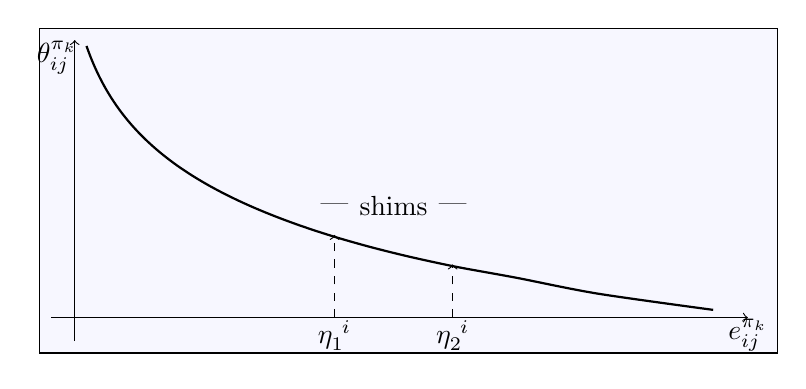
\begin{tikzpicture}[scale=0.75, samples=100]
			\filldraw[fill=blue!3!white, draw=black] (0, 0) rectangle (12.5, 5.5);
			\draw[->] (.2, .6) -- coordinate (x axis mid) (12, .6);
			\node at (5, 0.3) {$\eta_1^{\ i}$};
			\node at (5, 2.5) {|};
			\node at (6, 2.5) {shims};
			\node at (7, 2.5) {|};
			\node at (7, 0.3) {$\eta_2^{\ i}$};
			\node at (0.3, 5) {$\theta_{ij}^{\pi_k}$};
			\draw[->] (.6, .2) -- coordinate (y axis mid) (0.6, 5.3);
			\node at (12, 0.3) {$e_{ij}^{\pi_k}$};
			\draw[smooth, domain = 0.09:2, color=black, thick] plot (.3+1/\x,{4.2+log2(\x)});
			\draw[->, dashed] (5, 0.6)--(5, 2.0);
			\draw[->, dashed] (7, 0.6)--(7, 1.5);
		\end{tikzpicture}
		
		\captionof{figure}{$n^{\pi_k}$\/ edges $e_{ij}^{\pi_k}$\/ of $p_i$\/ sorted by $\theta_{ij}^{\pi_k}$\/ in non-ascending order}
		\label{fig:whip}		
	\end{minipage}
\end{table}


Figure \ref{fig:whip} represents the $n^{\pi_k}$\/ possible edges $e_{ij}^{\pi_k}$\/ of $i$\/ sorted by $\theta_{ij}^{\pi_k}$. \emph{Shims}\/ starts with a greedy solution, stopping at the edge with index $\eta_1^i$ (first phase). Then, considering even the edge with the index $\eta_2^i$, it elaborates different possible complements for this pallet (second phase) and selects the best of these complements (third phase).

In this heuristic, described in Algorithm \ref{alg:shims}, pallets $i$\/ are considered in non-descending order of $|D_i^{long}|$ (line \ref{shims:pallets}). For each pallet, the $n^{\pi_k}$\/ possible edges $e_{ ij}^{\pi_k}$\/ are considered in non-increasing order of $\theta_{ij}^{\pi_k}$\/ (line \ref{shims:possible}) in three phases: the greedy phase (until line \ref{shims:endfirst}), the composition phase of the shims (lines \ref{shims:beginsecond}-\ref{shims:endsecond}) and the selection phase of the best shim (lines \ref{shims:beginthird}-\ref{shims:endthird}).

{\color{blue}
	In the beginning of the first phase (line \ref{shims:initQ}), the set $Q^{\pi_k}$ represents the PC whose destination is not $\pi_k$, the current node, thus remaining on board.
	
	It is important to remember that $Q^{\pi_k}$ and $M$ were modified by the procedures $UpdatePacked(M, Q^{\pi_k}, \pi_k)$ and $SetPalletsDestinations(M, \pi_k)$, having their positions and destinations reassigned.
	
	Until line \ref{shims:endfirst}, a greedy and partial solution for pallet $i$ is constructed by edges inclusion, until a certain volume limit ($V_i \times limit$) is reached.
	The value of the {\it limit} (0.92) was empirically determined by the {\it iRace} tool developed by \cite{LopezIbanezManuel2016}.
	
	In the second phase (lines \ref{shims:beginsecond} to \ref{shims:endsecond}), a set of shims named $Set$\/ is created, where each {\it Shim} is formed by a set of edges in the range $[\eta_1^i,\eta_2^i]$, whose total volume is limited by $slack_i$. In this phase, the heuristic that provided the best results, both in terms of time and quality, is based on {\it First-Fit Decreasing}, which is an approximation algorithm for the {\it Bin Packing Problem}\/ \cite{JohnsonGarey1985}. Basically, shims are created by accumulating the following edges, taking $slack_i$\/ as a limit.
	
	In the third phase (lines \ref{shims:beginthird}-\ref{shims:endthird}), the best {\it Shim} in the $Set$\/ is chosen. Initially, two shims are found: $sh_w$\/ with larger weight and $sh_v$\/ with larger volume. Among the two, the {\it Shim} with the highest score will be chosen and its edges are inserted into $E^M_{N^{\pi_k}}$.
}

\begin{algorithm}[H]
	\caption{$Shims$\/ heuristic on node $\pi_k$}  \label{alg:shims}
	\begin{algorithmic}[1]
		
		\Procedure{$SolveNode$}{$Shims,\ \pi_k,\ G$}
		
		\State $G(M \cup N^{\pi_k} \cup Q^{\pi_k}, E^M_{Q^{\pi_k}})$ \Comment{a graph with pallets positions ($M$), PC ($Q^{\pi_k}$), and edges ($E^M_{Q^{\pi_k}}$)}  \label{shims:initQ}
		
		\State Sort $M$ by $|D_i|$ in non-descending order \label{shims:pallets}
		
		\State $E^M_{N^{\pi_k}} \gets \{\ \}$  \Comment{an empty set of pallet-item edges}
		
		\State Let $E_{ij}$ be an array with $m \times n^{\pi_k}$ edges $(i,\ j)$ sorted by $\theta_{ij}^{\pi_k}$ in non-ascending order \label{shims:possible}
		
		\State $\tau^{\pi_k} \gets 0$	 \Comment{aircraft torque in node $\pi_k$}	
		\State $\tau_{max} \gets W_{max} \times limit^{CG}_{long}$ \Comment{maximum aircraft torque}
			
		\State $volume \gets \{0\ |\ [1,2,3,...,m] \}$
		\State $slack  \gets \{0\ |\ [1,2,3,...,m] \}$
		
		\State $limit \gets 0.92$ \Comment{0.92 was obtained by the {\it iRace} package \cite{LopezIbanezManuel2016}}
		
		\For{$i \in \{1,2,3,...,m\}$}
					
			\For{$q \in \{1,2,3,...,m^{\pi_k}\}$}
			
				\If{$(i, q) \in E^M_{Q^{\pi_k}}$} 
					\State $volume_i \gets volume_i + v_q$ 
				\EndIf		
			\EndFor	
			
			\For {$e_{ij} \in E_{ij}$}
				
				\State $\Delta\tau \gets w_j \times D_i$
				
				\State $\tau_{new} \gets | \tau^{\pi_k} + \Delta\tau |$
				
				\If{ ($E^M_{N^{\pi_k}} \cup \{e_{ij}\}$ is feasible) {\bf and} ($volume_i \leq V_i \times limit$) {\bf and} ($\tau_{new} \leq \tau_{max}$ )} 
				
					\State $E^M_{N^{\pi_k}} \gets E^M_{N^{\pi_k}} \cup \{e_{ij}\}$
					
					\State $volume_i \gets volume_i + v_j$
					
					\State $\eta_1^{\ i} \gets \eta_1^{\ i} + 1$ 
					
					\State $\tau^{\pi_k} \gets \tau^{\pi_k} + \Delta\tau$
				
				\EndIf
				
			\EndFor			 \Comment{end of the first phase} \label{shims:endfirst}	
				

			\State $slack_i \gets V_i - volume_i$  \label{shims:beginsecond}
			\State $\eta_2^{\ i} \gets \eta_1^{\ i}$
			
			\Repeat
				\State $\eta_2^{\ i} \gets \eta_2^{\ i} + 1$  \label{shims:eta2}
				
				\State $e_{ij} \gets E_{i,\eta_2^{\ i}}$
				
				\State $volume_i \gets volume_i + v_j$
				
			\Until{($\eta_2^{\ i} = n^{\pi_k}$) {\bf or} ($ volume_i \geq (1 + 3 \times (1-limit)) \times V_i)$)} \label{shims:endsecond} \Comment{end of the second phase}
			

			\State $volume \gets 0$	\label{shims:beginthird}
			
			\State $volume \gets 0$, $b \gets 1$ $shims_b \gets \{\}$, $Set \gets Set \cup \{shims_b\}$
			
			\State $shims_b \gets \{\}$  \label{empty_shims}
			
			\State $Set \gets Set \cup \{shims_b\}$ \label{empty_set}
			
			\For{$x \in \{\eta_1^{\ i},...,\eta_2^{\ i} \}$} \label{edges_indexes}
			
			
				\State $NewShims \gets$ {\bf True} \label{new_shims}
				\State $e_{ij} \gets E_x^{\ i}$
				
				\For{$shims \in Set$} \label{shims_set}
				
					\If { $e_{ij} \not\in (E^M_{N^{\pi_k}} \cup shims)$ {\bf and} $e_{ij}$ is feasible  {\bf and}  $(v_j + volume) \leq slack_i$}
					
						\State $shims \gets shims \cup \{\ e_{ij}\ \}$
						\State $volume \gets volume + v_j$
						\State $NewShims \gets$ {\bf False} \label{new_shims_false}
						
						\State {\bf break}
					\EndIf
				
				\EndFor 
			
				\If{$NewShims$} \label{new_shims2}
					\State $volume \gets 0$
					\State $b \gets b + 1$
					\State $shims_b \gets \{\ \}$
					\State $shims_b \gets shims_b \cup \{e_{ij}\}$
					\State $Set \gets Set \cup \{\ shims_b\ \}$
				\EndIf
			
			\EndFor 
			
			\State $sh_w \gets shims$, where $shims \in Set$ and $\sum_{e_{ab} \in shims} w_b$ is maximum  \label{best_weight}		
			\State $sh_v \gets shims$, where $shims \in Set$ and $\sum_{e_{ab} \in shims} v_b$ is maximum \label{best_volume}
			\State $sh_{best} \gets shims$, where $shims \in \{sh_w, sh_v\}$ and $\sum_{e_{ab} \in x} s_b$ is maximum \label{best_score}
			
			\State $E^M_{N^{\pi_k}} \gets E^M_{N^{\pi_k}} \cup sh_{best}$ 	\label{shims:endthird}   \Comment{end of the third phase}

		\EndFor
		
		\Return $G(M \cup N^{\pi_k} \cup Q^{\pi_k}, E^M_{Q^{\pi_k}} \cup E^M_{N^{\pi_k}})$
		
		\EndProcedure
	\end{algorithmic}
\end{algorithm}


\section{Implementation and results}
\label{sec6}

This section is composed of two parts: the generation of test instances and the results obtained in our implementation.


\subsection{Instances generation}
\label{items}

As we are dealing with a new problem, which until now had not been modeled in the literature, we have to create our own benchmarks. For this, we based on the characteristics of real airlifts carried out by the {\it Brazilian Air Force}, as described below.

In the military airlift carried out in Brazil from 2008 to 2010, 23\% of the items weighed between $10kg$ and $20kg$, 22\% from $21kg$ to $40kg$, 24\% from $41kg$ to $80kg$, 23\% from $81kg$ to $200kg$, and 8\% between $201kg$ and $340kg$. These five groups of items are described in Table \ref{tab:weights}, where $P$\/ represents the group probability. On the other hand, the average density of these items is approximately $246 kg/m^3$.

\begin{table}[H]
	\centering
	\caption{Items weight distribution ($kg$) in Brazil}  \label{tab:weights}
	\begin{tabular}{c c c c }
		\toprule
		$Group$ & $P$ & $low$ & $high$  \\		
		\midrule
		1              & 0.23           & 10  & 20  \\
		2              & 0.22           & 21  & 40  \\
		3              & 0.24           & 41  & 80  \\		
		4              & 0.23           & 81  & 200 \\
		5              & 0.08           & 201 & 340 \\
		\bottomrule
	\end{tabular}
\end{table}


In the generation of test instances, we use three types of random selections:
\begin{itemize}
	\item $RandomReal(r_1,r_2)$: randomly selects a real number in $[r_1,r_2]$, where $r_1$ and $r_2$ are real numbers;
	\item $RandomInt(i_1,i_2)$: randomly selects a integer number in $[i_1,i_2]$, where $i_1$ and $i_2$ are integer numbers;
	\item $Roulette(set)$ biased through $\phi$: selects an element from $set$, where the probability of each element is proportional to the value of a given function $\phi$\/ defined on $set$.
\end{itemize}

\begin{algorithm}[H]
	\caption{Procedure to generate items}  \label{alg:itemsgen}
	\begin{algorithmic}[1]
		
		\Procedure{$ItemsGeneration$}{$scenario,\ volume$}
		
		\State Let $L$ and $M$ be according to $scenario$ \label{ig:LM}
		\State $limit \gets volume \times \sum_{i=1}^{m} V_i$ \label{ig:extended}
		
		\State Let $t_j^k$ be an item $j$ in node $k$.
		
		\For{$k \in \{0,1,2,...,K\}$}
		
			\State $N_k \gets \{\ \}$
			\State $j \gets 0$
			\State $vol \gets 0$	\label{ig:totals}	
			\While{$vol < limit$}
			
				\State $j \gets j+1$
				
				\Repeat
					\State $to_j \gets RandomInt(0, K)$ \label{ig:dest}
				\Until{$to_j \neq k$}
				
				\State $x = Roulette(item)$ biased through $P$ \label{ig:weight1} \Comment{From Table \ref{tab:weights}}
					
				\State $w_j \gets RandomReal(low(x), high(x))$        \label{ig:weight2}		
				
				\State $s_j \gets \round{100 \times (1 - \log_{10}(RandomInt(1, 9)))} $ \label{ig:score}
				
				\State $v_j \gets w_j / RandomReal(148, 344)$ \label{ig:volume}
				
				\State $vol \gets vol + v_j$ 
				
				\State $N_k \gets N_k \cup \{t_j^k\}$ 
			\EndWhile

		\EndFor
		
		\State $N \gets \bigcup_{0 \leq k \leq K} N_k$
		
		\Return $N$
		
		\EndProcedure
	\end{algorithmic}
\end{algorithm}

$ItemsGeneration$, which generates $N$, is described in Algorithm \ref{alg:itemsgen}. The parameter $scenario$\/ defines $L$\/ and $M$\/ (line \ref{ig:LM}), and the parameter $volume$\/ sets a limit on the total volume of items at each node (line \ref{ig:extended}). To avoid simply loading all items, we use $volume > 1$ {\color{blue}(1.2, 1.5, and 2.0). This represents more test instances for each scenario.}

For each generated $t^k_j$\/ item, its destination is randomly selected (line \ref{ig:dest}), its weight has a distribution according to Table \ref{tab:weights} (lines \ref{ig:weight1}-\ref{ig:weight2}), its score varies $100$\/ (highest) and $5$\/ (lowest) according to a logarithmic scale (line \ref{ig:score}, and its volume is randomly defined from the density, where we allow a variation of 40\% more or less than the average density of $246 kg/m^3$\/ (line \ref{ig:volume}).

{\color{blue}

\subsection{Results obtained}

In the tests performed, we used a 64-bit, 16GB, 3.6GHz, eight-core processor with {\it Linux Ubuntu 22.04.1 LTS 64-bit} as the operational system and {\it Python 3.10.4}\/ as the programming language. We also used the well-known solver {\it Gurobi}\/ (www.gurobi.com), version 9.5.2.

We ran Algorithm \ref{alg:main} in the 5 scenarios described in Table \ref{tab:scenarios}, considering 6 methods for node-by-node solution: Gurobi (see \ref{solver}), ACO, NMO, TS, GRASP, and Shims (Algorithm \ref{alg:shims}). In generating the items in each node, we consider 3 values for the parameter $volume$. The results obtained for the function $f$, with the corresponding run time in seconds, are shown in Tables \ref{tab:20} ($volume = 1.2$), \ref{tab:50} ($volume = 1.5$) and \ref{tab:100} ($volume = 2.0$). For each $method$, $scenario$\/ and $volume$, 7 different instances were generated. Therefore, 105 tests (5 scenarios $\times$\/ 3 volumes $\times$\/ 7 instances) were performed for each method. 

The average values were presented for $f_{\pi}$\/ and, for the run time, the worst result obtained. To facilitate the comparison between the methods, we added a last column in these tables, where two values are indicated:
\begin{itemize}
	\item {\bf Normalized}: value between 0 and 1, which corresponds to the ratio between the sum of $f$\/ values obtained by the method in all scenarios and the sum of the best values obtained among all methods in all scenarios. The higher the value of {\bf Normalized}, the closer the method approached the best solutions found.
	\item {\bf Speed-up}: ratio of the sums of the worst runtimes of all scenarios and the sum of the method runtimes in all scenarios. The method with the highest {\bf Speed-up}\/ is the fastest.
\end{itemize}

In each $scenario$, we indicate in bold the best value of $f$\/ found. In each table, we also indicate in bold the best {\bf Normalized}\/ and {\bf Speed-up}\/ values.


\begin{table}[H]
	\centering
	\caption{Methods and scenarios with $volume =1.2$}  \label{tab:20}
	\footnotesize
	\begin{tabular}{c|c|ccccc|c}
		\toprule
		{$method$}                        & {\bf Results}    & {\bf 1}     &  {\bf 2}    & {\bf 3}      & {\bf 4}      & {\bf 5}  & \specialcell{{\bf Normalized}\\{\bf Speed-up}}  % 14.40	 184
		\\
		\toprule
		\multirow{2}{*}{\textbf{Gurobi}}  & $f$      & 8.03   & {\bf 12.02}& {\bf 13.15} & {\bf 14.40} & {\bf 0.00} & {\bf 0.997} \\ %51,84
		&{\bf run time (s)}                          & 14     & 20         & 73          & 184         & 1,044       &  1.000 \\ 
		\midrule[.1pt]
		\multirow{2}{*}{\textbf{TS}}      & $f$      & 6.56     & 8.49       & 9.19       & 11.25      & 11.48      &  0.906 \\
		&{\bf run time (s)}                          & 4       & 17        & 86        & 516       & 3,600     &  2.709 \\ 
		\midrule[.1pt]		
		\multirow{2}{*}{\textbf{GRASP}}   & $f$      & 6.76     & 8.85       & 9.65       & 11.75      & 11.54      &  0.937 \\ 
		&{\bf run time (s)}                          & 4       & 17        & 80        & 472       & 3,265     &  2.984 \\ 
		\midrule[.1pt]
		\multirow{2}{*}{\textbf{ACO}}     & $f$      & {\bf 6.77}& 8.85      & 9.65       & 11.75      & 11.54      &  0.937 \\ 
		&{\bf run time (s)}                          & 4        & 17       & 86        & 513       & 3,596     &  2.714 \\ 
		\midrule[.1pt]	
		\multirow{2}{*}{\textbf{NMO}}     & $f$      & 6.74      & 8.80      & 9.61       & 11.76      & 11.50      &  0.934 \\
		&{\bf run time (s)}                          & 4        & 17       & 86        & 508       & 3,480     &  2.796 \\ 
		\midrule[.1pt]	
		\multirow{2}{*}{\textbf{Shims}}   & $f$      & {\bf 6.77} & 8.92     & 9.60       & 11.78      & 11.61      &  0.939       \\ 
		&{\bf run time (s)}                          & 2         & 8       & 31        & 166       & 1,087     &  {\bf 8.856} \\ 
		\bottomrule
	\end{tabular}
	\normalsize
\end{table}



\begin{table}[H]
	\centering
	\caption{Methods and scenarios with $volume =1.5$}  \label{tab:50}
	\footnotesize
	\begin{tabular}{c|c|ccccc|c}
		\toprule
		{$method$}                        & {\bf Results}   & {\bf 1}     &  {\bf 2}    & {\bf 3}      & {\bf 4}      & {\bf 5}    & \specialcell{{\bf Normalized}\\{\bf Speed-up}} \\
		\toprule
		\multirow{2}{*}{\textbf{Gurobi}}  & $f$     & 4.756       & 8.84        & 11.94       & 16.21       &{\bf 16.47} & 0.852  \\	% 6828 
		&{\bf run time (s)}                         & 18        & 68         & 326        & 1,906      & 12,960    & 1.000  \\	 
		\midrule[.1pt]
		\multirow{2}{*}{\textbf{TS}}      & $f$     & 8.97       & 11.44       & 12.92       & 15.20       & 15.39      &  0.936 \\		
		&{\bf run time (s)}                         & 4         & 18         & 88         & 525        & 3,660     &  3.555  \\		
		\midrule[.1pt]		
		\multirow{2}{*}{\textbf{GRASP}}   & $f$     & 9.36       & 12.34       & 13.63       & 16.18       & 15.44      &  0.981 \\ 
		&{\bf run time (s)}                         & 4         & 17         & 86         & 515        & 3,564     &  3.651  \\
		\midrule[.1pt]	
		\multirow{2}{*}{\textbf{ACO}}     & $f$     & 9.36       & 12.34       & 13.63       & 16.18       & 15.44      &  0.981 \\
		&{\bf run time (s)}                         & 5         & 19         & 90         & 539        & 3,720     &  3.492  \\	
		\midrule[.1pt]	
		\multirow{2}{*}{\textbf{NMO}}     & $f$     & 9.36       & 12.33       & 13.60       & 16.16       & 15.43      &  0.979 \\ 
		&{\bf run time (s)}                         & 5         & 19         & 91         & 544        & 3,780     & 3.442  \\
		\midrule[.1pt]	
		\multirow{2}{*}{\textbf{Shims}}   & $f$     & {\bf 9.39} & {\bf 12.42} & {\bf 13.72} & {\bf 16.28} & 15.49      &  {\bf 0.986} \\	
		&{\bf run time (s)}                         & 3         & 11         & 48         & 265        & 1,720     &  {\bf 7.470}  \\
		\bottomrule
	\end{tabular}
	\normalsize
\end{table}


\begin{table}[H]
	\centering
	\caption{Methods and scenarios with $volume = 2.0$}  \label{tab:100}
	\footnotesize
	\begin{tabular}{c|c|ccccc|c}
		\toprule
		{$method$}                        & {\bf Results}    & {\bf 1}     &  {\bf 2}   & {\bf 3}    & {\bf 4}    & {\bf 5}      & \specialcell{{\bf Normalized}\\{\bf Speed-up}} \\
		\toprule
		\multirow{2}{*}{\textbf{Gurobi}}  & $f$              & 4.92      & 6.58      & 6.34       & 7.24       & 8.15      &  0.334 \\ % 9951
		                                  &{\bf run time (s)}& 29       & 106      & 493      & 2,833     & 19,380      &  1.000  \\ 
		\midrule[.1pt]
		\multirow{2}{*}{\textbf{TS}}      & $f$              & 13.72     & 17.53     & 19.28     & 21.78      & 22.35      &  0.951 \\		
		&{\bf run time (s)}                                  & 5        & 19       & 93       & 556       & 3,900     &  4.992  \\	
		\midrule[.1pt]		
		\multirow{2}{*}{\textbf{GRASP}}   & $f$        & 13.99     & 19.39     & 19.86     & 23.50      & 22.57      &  0.998 \\
		&{\bf run time (s)}                            & 6        & 21       & 97       & 571       & 3,960     &  4.906  \\	
		\midrule[.1pt]
		\multirow{2}{*}{\textbf{ACO}}     & $f$        & 13.99     & 19.39     & 19.86     & 23.50      & 22.57      &  0.998 \\
		&{\bf run time (s)}                            & 6        & 23       & 105      & 597       & 4,080     &  4.745  \\	
		\midrule[.1pt]	
		\multirow{2}{*}{\textbf{NMO}}     & $f$        & 13.99     & 19.39     & 19.85     & 23.50      & 22.56      & 0.998 \\	
		&{\bf run time (s)}                            & 9        & 27       & 120      & 681       & 4,620     & 4.184  \\	
		\midrule[.1pt]	
		\multirow{2}{*}{\textbf{Shims}}   & $f$        &{\bf 14.00} & {\bf 19.44} & {\bf 19.94} & {\bf 23.55} & {\bf 22.58} & {\bf 1.000} \\	
		&{\bf run time (s)}                            & 7        & 20       & 84       & 450       & 2,918     & {\bf 6.570}  \\
		\bottomrule
	\end{tabular}
	\normalsize
\end{table}

{\color{blue}
It is important to note that the best tour found in each test was seldom the tour with the lowest cost (the minimal cost tour without considering the CG deviation), but any of the first 25\% of the best tours. This indicates that our strategy of enumerating and solving all tours was assertive, although it is possible to devise a more proactive strategy to discard most of the higher-cost tours and improve performance. This must be one of the next steps in this research.

If a posterior application of this method requires 8, 9, or more nodes, it is possible to use this 25\% as a threshold to discard the higher-cost tours and keep the run time within an operational acceptable limit for the client.
}

In Tables \ref{tab:20}, \ref{tab:50} and \ref{tab:100}, $Gurobi$\/ was the slowest method and $Shims$\/ was the fastest. This was expected, as $Gurobi$\/ is a MIP solver, which seeks an optimal solution within the established constraints, usually reaching its time limit on each node, while {\it Shims} is a fast heuristic. This way, $Gurobi$\/ even demands prohibitive times (more than 5 hours in scenario 6 of Table \ref{tab:100}), while the maximum time required by $Shims$\/ did not reach one hour.

Considering the {\bf Normalized}\/ values, in Table \ref{tab:20} $Gurobi$\/ was the best ($0.997$), followed closely by $Shims$\/ ($0.939$). In Tables \ref{tab:50} and \ref{tab:100}, $Shims$ was the best ($0.986$\/ and $1.000$). As expected, the performance of $Gurobi$\/ drops sharply as the volume of shipments at the nodes increases: $0.852$\/ in Table \ref{tab:50} and $0.334$\/ in Table \ref{tab:100}.

It is worth noting that the other heuristics always obtained {\bf Normalized}\/ values greater than or equal to $0.9$, and were always faster than $Gurobi$.


	
It is not possible to state how far these results are from the optimal solutions, but we can report that all occupancy rates in terms of volume were above 97\%, and in terms of weight above 79\%, which denotes that the results achieved are good, considering that the CG deviation constraints keeps these values from going higher.


\subsubsection{Proposed strategy assessment}

Another important test is to compare the best tour score/cost ratio with the least expensive tour score/cost ratio. This is important to see how far our solution strategy is from the simplest form, just solving a TSP.

For this achievement, we ran {\it Shims} in 5 scenarios with 7 instances each, and 3 volume surpluses, collecting the averages of the best tour result and the least cost tour result.

\begin{table}[H]
\centering
\caption{Shims best and least cost tour results}  \label{tab:20least}
\footnotesize
\begin{tabular}{c|c|ccccc|cc}
\toprule
{$surplus$}              & {\bf Tour} & {\bf 1} & {\bf 2} & {\bf 3} & {\bf 4}  & {\bf 5}   & {\bf Sum} & {\bf Improvement}\\

\midrule[.1pt]	
\multirow{2}{*}{$1.2$}   & Least cost    & 6.23  & 11.56   & 12.88   & 13.54    & 12.47  & 56.68 &       \\ 
& Best                                   & 7.96  & 13.04   & 14.30   & 15.56    & 15.28  & 66.14 & 16.7\%  \\ 
\midrule[.1pt]	
\multirow{2}{*}{$1.5$}   & Least cost    & 8.44  & 16.61   & 18.18   & 19.68    & 17.64  & 80.55 &   \\ % 17.64	 20.94	
& Best                                   & 11.47 & 18.25   & 20.61   & 22.22    & 20.94  & 93.49 & 16.1\%  \\ 
\midrule[.1pt]	
\multirow{2}{*}{$2.0$}   & Least cost    & 13.38 & 22.46   & 25.97   & 26.23    & 22.51  & 110.55 &   \\ %22.51	 29.09
& Best                                   & 17.93 & 25.59   & 28.61   & 31.28    & 29.09  & 132.50 & 19.9\%  \\ 		                         

\midrule[.1pt]
 \multicolumn{8}{r}{{\bf Average improvement}} & 17.6\% \\
\bottomrule
\end{tabular}
\normalsize
\end{table}

As the selection of the best tour, considering what was collected and delivered in each node, and considering the cost increase due to CG deviation, was 17.6\% better than the option for a simple TSP solution (\textit{Least cost} results), this confirms that our solution strategy was adequate.

}

\section{Conclusions}
\label{sec7}

In this work, we modeled and solved a real air transport problem, named {\it Air Cargo Load Planning with Routing, Pickup and Delivery Problem}\/ (ACLP+RPDP). For the first time in the literature, a NP-hard problem that involves {\it simultaneously}\/ pallet assembly, load balancing and route planning is addressed, where the cost-effectiveness of transport is maximized. We adopted some simplifications that are not critical, but that allowed the unprecedented solution of this problem considering more than two nodes.

We consider that, in practical cases, the number $K$\/ of nodes, excluding the base, is small ($K \leq 6$), each of them with hundreds of items to be shipped. Thus, considering real aircraft models, we developed some node-by-node heuristics, which allow us to enumerate all $K!$\/ tours and choose the best. The complete process can be executed quickly on a simple handheld computer, offering good results and reducing stress for the transport planners. As validation, we performed tests in several scenarios with real data from the {\it Brazilian Air Force}.

In less than one hour, this development can establish a good distribution of load on pallets to be put in the cargo bay, enforcing the loaded aircraft balance, maximizing the total score and minimizing fuel consumption for the airlift. The output, which includes the tour plan and the pallet building and arrangement plan, is an essential part of airlift: it improves flight safety, makes ground operations more efficient, and makes sure that each item gets to its right destination.

Our main contributions were the mathematical modeling of this complex problem, which involves four NP-hard subproblems, and a complete process that offers a fast and good-quality solution.

{\color{blue}
As this is ongoing research, some improvements are possible, which are the next steps of the development:

(1) This work addresses all possible tours, but we plan bounding schemes to allow for discarding most of the higher-cost tours. This is expected to reduce the running time, favoring the discovery of better search mechanisms.

(2) We are also working on computer parallelism to accelerate the algorithms.

(3) In the event that these gains in performance are achieved, we strongly believe that they will permit the application of a 3-dimensional packing procedure to maximize the occupancy rate among the selected items.
}

The simple heuristic $Shims$\/ presented a resolution with the best node-by-node results in a restricted time interval. Without it, it would not be possible to test all routes: after all, the greater the number of nodes, the shorter the run time limit for node-by-node solution. We also show that, as the shipment volume increases, the exact node-by-node solution becomes unfeasible, indicating the importance of a fast and good-quality heuristic.

Finally, by focusing on node-by-node solution, the resolution of this work is not exclusive to aircraft and airports: it can be adapted, for example, to ships and ports, or vehicles and warehouses, or freight cars and railways. In these cases, it would be necessary to make some changes in the modeling: for example, modify the load balancing constraints, and consider the available space in vehicles or freight cars instead of pallets.


\section*{Acknowledgments}

This research was partially supported by \textit{S�o Paulo Research Foundation} (FAPESP, grant 2016/01860-1).

\begin{thebibliography}{00}

\bibitem{LarsenMikkelsen1979} O. Larsen and G. Mikkelsen, An interactive system for the loading of cargo aircraft, {\it European Journal of Operational Research}, Vol. 4 (6), pp. 367-373, 1980.

\bibitem{Brosh1981} Israel Brosh, Optimal cargo allocation on board a plane: a sequential linear programming approach, {\it European Journal of Operational Research}, Vol. 8 (1), pp. 40-46, 1981.

\bibitem{JohnsonGarey1985} D.S. Johnson and M.R. Garey, A 71/60 theorem for bin packing, {\it Journal of Complexity}, Vol. 1 (1), pp. 65-106, 1985.

\bibitem{Glover1986} Fred Glover, Future paths for integer programming and links to artificial intelligence, {\it Computers and Operations Research}, Vol. 13, pp. 533-549, 1986.

\bibitem{FeoResende1989} Thomas A. Feo and Mauricio G.C. Resende, A probabilistic heuristic for a computationally difficult set covering problem, {\it Operations Research Letters}, Vol. 8 (2), pp. 67-71, 1989.

\bibitem{Kevin1992} Kevin Y.K. Ng, A multicriteria optimization approach to aircraft loading, {\it Operations Research}, Vol. 40 (6), pp. 1200-1205, 1992.

\bibitem{Dorigo1992} Marco Dorigo, {\it Optimization, Learning and Natural Algorithms}, PhD Thesis, Politecnico di Milano, 1992.

\bibitem{CharonHudry1993} I. Charon and O. Hudry, The noising method: a new method for combinatorial optimization, {\it Operations Research Letters}, Vol. 14 (3), pp. 133-137, 1993.

\bibitem{DorigoManiezzoColorni1996} M. Dorigo, V. Maniezzo and A. Colorni, The ant system: optimization by a colony of cooperating agents, {\it IEEE Transactions on Systems, Man, and Cybernetics}, Vol. 26 (1), pp. 29-41, 1996.

\bibitem{NiarFreville1997} S. Niar and A. Freville, A parallel tabu search algorithm for the 0-1 multidimensional knapsack problem, Proceedings of {\it 11th International Parallel Processing Symposium}, 1997.

\bibitem{Heidelberg1998} K.R. Heidelberg, G.S. Parnell and J.E. Ames, Automated air load planning, {\it Naval Research Logistics}, Vol. 45 (8), pp. 751-768, 1998.

\bibitem{CharonHudry2001} I. Charon and O. Hudry, The noising methods: a generalization of some metaheuristics, {\it European Journal of Operational Research}, Vol. 135 (1), pp. 86-101, 2001.

\bibitem{MongeauBes2003} Marcel Mongeau and Christian Bes, Optimization of aircraft container loading, {\it IEEE Transaction on Aerospace and Electronic Systems}, Vol. 39 (1), pp. 140-150, 2003.

\bibitem{fok2004optimizing} Kelly Fok and Andy Chun, Optimizing air cargo load planning and analysis, Proceedings of {\it The International Conference on Computing, Communications and Control Technologies}, 2004.

\bibitem{Fidanova2006} S. Fidanova, Ant colony optimization and multiple knapsack problem and model bias, {\it Numerical Analysis and Its Applications}, Springer Berlin Heidelberg, pp. 280-287, 2005.

\bibitem{Chan2006} F.T.S. Chan, R. Bhagwat, N. Kumar. M.K. Tiwari and P. Lam, Development of a decision support system for air-cargo pallets loading problem: a case study, {\it Expert Systems with Applications}, Vol. 31 (3), pp. 472-485, 2006.

\bibitem{KaluznyBohdanL2009Oalb} B.L. Kaluzny and R.H.A.D. Shaw, Optimal aircraft load balancing, {\it International Transactions in Operational Research}, Vol. 16 (6), pp. 767-787, 2009.

\bibitem{MesquitaCunha2011} A.C.P. Mesquita and C.B. Cunha, An integrated heuristic based on the Scatter Search metaheuristic for vehicle routing problems with simultaneous delivery and pickup in the context of the Brazilian Air Force, {\it Transportes}, Vol. 19, pp. 33-42, 2011.

\bibitem{Verstichel2011} J. Verstichel, W. Vancroonenburg, W. Souffriau and G.V. Berghe, A mixed integer programming approach to the aircraft weight and balance problem, {\it Procedia Social and Behavioral Sciences}, Vol. 20, pp. 1051-1059, 2011.

\bibitem{Limbourg2012} S. Limbourg, M. Schyns and G. Laporte, Automatic aircraft cargo load planning, {\it Journal of the Operational Research Society}, Vol. 63 (9), pp. 1271-1283, 2012.

\bibitem{RoesenerHall2014} A.G. Roesener and S. Hall, A nonlinear integer programming formulation for the airlift loading problem with insufficient aircraft, {\it Journal of Nonlinear Analysis and Optimization: Theory and Applications}, Vol. 5 (1), pp. 125-141, 2014.

\bibitem{Vancroonenburg2014} W. Vancroonenburg, J. Verstichel, K. Tavernier and G.V. Berghe, Automatic air cargo selection and weight balancing: a mixed integer programming approach, {\it Transportation Research Part E: Logistics and Transportation Review}, Vol. 65, pp. 70-83, 2014.

\bibitem{LurkinSchyns2015} V. Lurkin and M. Schyns, The airline container loading problem with pickup and delivery, {\it European Journal of Operational Research}, Vol. 244 (3), pp. 955-965, 2015.

\bibitem{RoesenerBarnes2016} A.G. Roesener and J.W. Barnes, An advanced tabu search approach to the dynamic airlift loading problem, {\it Logistics Research}, Vol. 9 (1), pp. 1-18, 2016.

\bibitem{PaquaySchynsLimbourg2016} C. Paquay, M. Schyns and S. Limbourg, A mixed integer programming formulation for the three-dimensional bin packing problem deriving from an air cargo application, {\it International Transactions in Operational Research}, Vol. 23 (1-2), pp. 187-213, 2016.

\bibitem{PaquayLimbourgSchynsOliveira2018} C. Paquay, S. Limbourg, M. Schyns and J.F. Oliveira, MIP-based constructive heuristics for the three-dimensional bin packing problem with transportation constraints, {\it International Journal of Production Research},
Vol. 56 (4), pp. 1581-1592, 2018.

\bibitem{Laabadi2018} S. Laabadi, M. Naimi, H. El Amri and B. Achchab, The 0/1 multidimensional knapsack problem and its variants: a survey of practical models and heuristic approaches, {\it American Journal of Operations Research}, Vol. 8, pp. 395-439, 2018.

\bibitem{YangLiuGao2018} Y. Chenguang, L. Hu and G. Yuan, Load planning of transport aircraft based on hybrid genetic algorithm, {\it MATEC Web of Conferences}, Vol. 179, pp. 1-6, 2018.

\bibitem{Alonso2019} M.T. Alonso, R. Alvarez-Valdes and F. Parreno, A GRASP algorithm for multi-container loading problems with practical constraints, {\it A Quarterly Journal of Operations Research}, Vol. 18, pp. 49-72, 2019.

\bibitem{BrandtStefan2019} F. Brandt and S. Nickel, The air cargo load planning problem - a consolidated problem definition and literature review on related problems, {\it European Journal of Operational Research}, Vol. 275 (2), pp. 399-410, 2019.

\bibitem{wong2020} E.Y.C. Wong and K.K.T. Ling, A mixed integer programming approach to air cargo load planning with multiple aircraft configurations and dangerous goods, Proceedings of {\it 7th International Conference on Frontiers of Industrial Engineering}, 2020.

\bibitem{Zhan2020} S. Zhan, L. Wang, Z. Zhang and Y. Zhong, Noising methods with hybrid greedy repair operator for 0-1 knapsack problem, {\it Memetic Computing}, Vol. 12, pp. 37-50, 2020.

\bibitem{eugene2021} E.Y.C. Wong, D.Y. Mo and S. So, Closed-loop digital twin system for air cargo load planning operations, {\it International Journal of Computer Integrated Manufacturing}, Vol. 34 (7-8), pp. 801-813, 2021.

\bibitem{zhao2021} X. Zhao, Y. Yuan, Y. Dong and R. Zhao, Optimization approach to the aircraft weight and balance problem with the centre of gravity envelope constraints, {\it IET Intelligent Transport Systems}, Vol. 15 (10), pp. 1269-1286, 2021.

\bibitem{LopezIbanezManuel2016} L�pez-Ib��ez, Manuel and Dubois-Lacoste, J�r�mie and P�rez C�ceres, Leslie and Birattari, Mauro and St�tzle, Thomas. 2016. The irace package: Iterated racing for automatic algorithm configuration. Elsevier. pp. 43-58. Volume 3.


\end{thebibliography}


\end{document}
